\documentclass[]{final}
\usepackage{graphicx, caption, subcaption, float, wrapfig}
\usepackage{cite, hyperref, xurl, xcolor, color}
\hypersetup{colorlinks=true, urlcolor=blue, citecolor=blue, linkcolor=black}
\usepackage{upgreek, amsmath, tipa , textcomp, amssymb}
\usepackage{listings, chapterbib, enumerate}
\usepackage[smartEllipses]{markdown}
\bibliographystyle{alpha}
\bibstyle{alpha}
\usepackage{tocloft}
\setlength\cftparskip{2pt}
\setlength\cftbeforechapskip{0pt}
\setlength\cftbeforesecskip{2pt}
\setlength\cftaftertoctitleskip{10pt}
\setlength{\cftbeforetoctitleskip}{-2em}
\newcommand{\bulletPoint}{\hspace{-3.1pt}$\bullet$ \hspace{5pt}}


\lstdefinestyle{mycodestyle}{
    basicstyle=\ttfamily,
    breakatwhitespace=false,
    breaklines=true,
    captionpos=b,
    keepspaces=true,
    numbers=left,
    numbersep=5pt,
    showspaces=false,
    showstringspaces=false,
    showtabs=false,
    tabsize=2
}
\lstset{style=mycodestyle}

%--
%submit as NAME.final.pdf
%The project demonstration will be assessed by the second marker


%TODO

%check vid demo & improve
%port-forward for demo - raspi as nginx, demo video like before but add new info. & new game

%structure of your directory, & interesting files for pong and zarlasht

%fix bibliography formatting



%logging - improvements, time, etc. - possible improvements but not priority

%---

\def\studentname{Faeq Faisal}
\def\reportyear{2025}
\def\projecttitle{A concurrency based game environment}
\def\supervisorname{Dr Julien Lange}
\def\degree{BSc (Hons) in Computer Science (Software Engineering)}
\def\fullOrHalfUnit{CS3821 Full Unit}
\def\finalOrInterim{Final Report}

%---

\begin{document}
\maketitle

%---

\chapter*{Declaration}
This report has been prepared on the basis of my own work. Where other published
and unpublished source materials have been used, these have been acknowledged.
\vskip3em
Word Count: \input{wordcount.txt}words
\vskip3em
Student Name: \studentname
\vskip3em
Date of Submission: Friday 4th April 2025
\vskip3em
Signature:
\vskip0em
\includegraphics[width=3cm]{faeq_faisal_signature}

\newpage

\tableofcontents\pdfbookmark[0]{Table of Contents}{toc}\newpage

\begin{abstract}

  \phantomsection
  \label{rationale_abstract}

  Playing games has become an integral part of modern society, offering not only entertainment but
  also serving as a tool for relaxation and stress relief, while simultaneously fostering critical thinking,
  and problem-solving skills. For certain demographics, such as individuals with disabilities who may have
  limited social interactions, or children still developing, games can provide unique benefits. These include
  learning important social skills like turn-taking, developing emotional intelligence, and building
  resilience~\cite{garaigordobil_developing_2022}. To add, the interactive nature of games, particularly those
  that provided multiplayer experiences, can foster social connections and enhance enjoyment for players;
  "fun experienced when interacting with others is more positive than solitary fun"~\cite{reis_fun_2017}.

  Multiplayer games significantly increase gamers' immersion and enjoyment~\cite{berladean_effect_2016}, but
  this experience hinges on the critical need for leveraging concurrency mechanisms, particularly within games that
  support simultaneous play across multiple game instances.
  These can be provided by programming
  languages, runtime environments or other technologies. These concurrency
  mechanisms can facilitate simultaneous actions in board games, provide real-time
  error reporting, support real-time chat systems that run alongside gameplay, and dynamic world
  updates across multiple clients. These capabilities, among others, enhance the responsiveness and
  interactivity of multiplayer game environments.

  To begin this project, I explored various concurrent environment technologies
  and architectures, ultimately selecting Gleam, targeting Erlang to run on the BEAM, for its
  robust, highly concurrent and fault-tolerant runtime. I developed multiple proof-of-concept
  programs, including an online chat system, Tic-Tac-Toe, and Pong, to experimentally validate
  the modularity and integration of my chosen technologies. These prototypes demonstrated
  the ability to support multiple simultaneous game instances, simultaneous game actions
  and real-time communication.

  I then investigated innovative concurrency-based features, like real-time world
  updates and 'racing' actions, for my final game, focusing
  on creating a flexible game environment that can support non-turn-based interactions.
  I also worked to address challenges in system reliability, including
  strategies for error handling and scalability, like using supervisors that
  can pass state from older children to younger ones.

  The aim of this report is to document my process of building a game environment for
  high-concurrency, providing a comprehensive overview of the design challenges,
  implementation strategies, and key technical achievements.
\end{abstract}

\newpage

\section{Original Project Specification}

\textbf{Aims:} The aim of the project is to develop a game-playing environment
using a programming language such as Java. Besides providing appropriate error reports,
the system should have a nice graphical interface and provide such advanced
features such as allowing multiple games to be played at the same time.

\textbf{Background:} Game-playing environments are popular systems with a
variety of functionalities. For example, such an environment usually allows
multiple games to be played at the same time. This can be implemented by means
of the concurrency mechanisms supported in a programming language: multiple games
are implemented as different threads that share the same modules that provide
the basic functionalities such as moves in board games and error reporting procedures.

\textbf{Early Deliverables}
\begin{enumerate}
  \item Proof of concept program: A prototype implementation of a board game (e.g., chess).
  \item Proof of concept program: A prototype program that exhibits the behaviour of concurrent execution.
  \item Report: A survey report on game environments.
  \item Report: A description of the prototype implementations.
\end{enumerate}

\textbf{Final Deliverables}
\begin{enumerate}
  \item The system must be implemented according to modern software engineering principles.
  \item The environment should contain a working system, with functionalities such as error reporting.
  \item A graphical interface should be implemented.
  \item The environment should allow the users to play multiple games at the same time.
  \item The report should provide an overview of game-playing environments.
  \item The report should describe the environment including its functionalities and design.
  \item The report should describe the implementation issues (such as the choice of data structures, numerical methods etc) necessary to apply the theory.
  \item The report should describe the testing procedures of the environment.
  \item The report should describe the software engineering process involved in the design and implementation.
\end{enumerate}

\textbf{Suggested Extensions}
\begin{itemize}
  \item Advanced GUI with other useful features such as chat room.
  \item Advanced implementation issues such as multiple game playing based on concurrency and sharing.
\end{itemize}

\textbf{Prerequisites:} Good command of programming languages such as Java.


\chapter{Introduction}
\section{The Problem}

\phantomsection
\label{rationale_problem}

Modern environments face significant challenges, especially in maintaining
system reliability and scalability, struggling to provide a responsive gameplay
experience. For example, the challenge of 'flash crowds', managing sudden user influxes,
can quickly transform a popular service into an unintentional victim of a
DDOS attack. "Flash crowds often cause very poor performance
at the server side and result in a significant number of unsatisfied
clients"\cite{Ari_crss_nodate}. Unexpectedly high, concurrent connections can overwhelm
system resources and cause catastrophic service failure, as was the case for
the CodinGame platform, where heavy loads led to a memory leak on the application
servers, and contributed towards a system crash\cite{jobert_story_2017}.

To support simultaneous game instances and multi-player interactions,
a robust concurrency model is essential. My approach initially involved
transitioning from more familiar technologies, like JavaScript, to
gradually understand and implement advanced concurrency concepts,
allowing for an exploration of new models and design patterns before
undertaking a more comprehensive architectural implementation.

After reviewing several concurrency models,
I found that actor-based concurrency would be best for my use-case.
As a result, I moved to using Erlang's implementation in OTP.
I reimplemented the prototypes in JavaScript, and created an additional
prototype, a game of Pong, to get comfortable.
I then moved to a final game that has advanced concurrency
features. I optimized reusable components from the prototypes to form the
base of the final game, and added to them to allow, for e.g., better system
reliability.

\section{Aims and Goals of the Project}
The primary aim of this project was to develop a concurrent game environment that;
\begin{enumerate}
  \item Supports multiple simultaneous game instances
  \item Enables real-time communication and dynamic world updates
  \item Provides a flexible, modular architecture for hosting different game types
  \item Demonstrates innovative concurrent programming techniques
  \item Implements robust error handling and system reliability mechanisms
  \item Has a nice graphical interface with error reporting
  \item Is implemented according to modern software engineering principles
\end{enumerate}

\newpage

\phantomsection
\label{rationale_importance}

The growing importance of multiplayer and interactive gaming experiences served
as the motivation for this project. After researching limitations in existing
game environment architectures, exploring the potential of advanced
concurrency models to enhance game interactivity, and evaluating different
approaches to distributed system design, I established the following goals
for last term;

\begin{enumerate}
  \item Produce a survey report on game environments
  \item Learn how WebSockets work and how to use them effectively
  \item Learn the functional programming paradigm through the Gleam programming language
  \item Learn how to use databases based off Redis OSS, like Valkey or DragonflyDB
  \item Design a scalable client-server model
  \item Implement my planned Online Chat and Tic-Tac-Toe proof of concepts in Gleam, targeting JavaScript, utilizing the above technologies
  \item Implement my planned Online Chat and Tic-Tac-Toe and Pong proof of concepts in Gleam, targeting Erlang, to learn it's concurrency model
  \item Ensure all code is well tested and documented for future reuse and adaptation
  \item Implement the foundational concurrent features for the final game
\end{enumerate}

In addition to designing a scalable environment,
by exploring the Erlang ecosystem, with its actor model representing one of the
most sophisticated approaches to concurrent programming, and
BEAM languages, particularly Gleam, a new, modern, statically-typed language,
this project aimed to address the limitations of existing multiplayer
game systems and create a more responsive game environment.

Throughout the first term, I successfully completed all planned objectives,
including developing the proof-of-concept applications,
establishing the core game environment architecture, and implementing initial
concurrent features for the final game. Anticipating the project timeline,
I had also began the next term's objectives, conducting comprehensive performance
optimizations and initiating informal user testing and feedback integration,
which allowed for earlier refinement of the system's design and functionality.

For the second term, I had the main objective of creating the final game, with
advanced concurrency features, which showcases all that I have learnt during the
project. This was broken down into the following objectives;

\begin{enumerate}
  \setcounter{enumi}{9}
  \item Produce a polished GUI for the game
  \item Implement niceties and useful features like the chat room
  \item Implement more advanced concepts;
        \begin{itemize}
          \item overriding actions in progress (players choosing a color)
          \item 'racing' actions (taking the first action to settle as a value)\\(players in a fight scenario)
          \item time limits for actions (players in a fight scenario)
          \item compound actions (players in a fight scenario)
          \item real-time dynamic world updates (viewing the map)
        \end{itemize}
  \item Implement further enhancements to reliability \& error handling\\(e.g., restoring state after a disconnection)
  \item Ensure all code is well optimized, tested and documented
  \item User testing and Address feedback
\end{enumerate}

\phantomsection
\label{successful}

This project was very successful, in that it met all of my objectives,
though some objectives, such as being "well" optimized, tested, and documented, are
inherently subjective. While I did make significant
improvements to, for e.g., error handling,
there are further actions that I could have taken, given time.
These will be outlined in greater detail later in the report.

\section{Rationale}

\phantomsection
\label{rationale}

As previously mentioned {\hypersetup{linkcolor=teal}(\pageref{rationale_importance}, \pageref{rationale_problem},
    and \pageref{rationale_abstract})},
the motivation for this project stems from the
rapidly evolving landscape of multiplayer, interactive gaming experiences,
and their importance in the modern day.
As the industry continues to grow, the need for scalable,
efficient, and concurrent game environments has become increasingly
critical, with pre-existing architectures used by large companies
being swapped out for ones that better suite the need (detailed later).
This project aims to address this demand by leveraging
state-of-the-art technologies and architectures
to create a robust and scalable game environment.
Focusing on concurrency
mechanisms and on what features can be developed from them, the project
not only aligns with current industry trends but
also challenges conventional constraints in real-time multiplayer games.

In terms of my future career in software engineering, this project is all-around a comprehensive learning experience that will undoubtedly enhance my adaptability and technical proficiency.
My use of unfamiliar technologies such as Gleam, Erlang, and Valkey, has provided me with a deep understanding of a variety of concepts including functional programming, actor based concurrency, asynchronous messaging, etc. .
To add, my use of HTMX for a dynamic, stateless, web interface and NGINX for efficient load balancing has given me hands-on
experience with modern web technologies and server management.

The architecture of the project, particularly my use of Pub/Sub with a pool of servers, has also been extremely insightful.
This approach allowed me to explore distributed systems and real-time communication; key topics within the field.
By both, designing and implementing the entire project from scratch, I have gained an invaluable experience in system design, problem-solving, and the ability to work with a diverse set of tools and frameworks.

Overall, this project not only addresses a pressing industry requirement but also provides
me the technical expertise and flexibility necessary to be successful in my future career.
ranging from learning new programming languages to designing scalable architectures, will enable me to
seamlessly adapt to new technologies and challenges in the workplace, rendering me as a more
versatile and capable software engineer.

\newpage

\addcontentsline{toc}{section}{Technology Choices}
\subsection{Technology Choices}

\phantomsection
\label{alpine}

For the front-end, the client-side, I used web technologies so that the Project
would be more accessible to all. For functionality, I mostly used HTMX,
but also added minimal JavaScript and Alpine.js, a lightweight JavaScript
framework for my final game. %TODO - CITE
This was mostly to allow me to focus on the
architecture of the environment and the implementation of the game
servers, as HTMX allows me to dynamically update the client-side, while
keeping it completely stateless for simplicity. As for my little use of
JavaScript and Alpine.js, these were mainly used to help produce a polished
GUI for the final game. While Alpine.js also helped with state management,
it never effected server state; the state of Alpine.js data was always
localized, and never effected functionality needed for the actual interactions
in the game, meaning that they could not bottleneck concurrency-based tasks.
For e.g., Alpine.js helped the user switch between system, light and dark
themes for the game, but the server was always unaware of what theme the user
was using as it did not require such information.

\phantomsection
\label{REDISOSS}

For the game servers themselves, I used Gleam, a new, type-safe, modern
language with comprehensive tooling built-in. I believe they described why I
chose their language best; "The power of a type system, the expressiveness
of functional programming, and the reliability of the highly concurrent,
fault tolerant Erlang runtime, with a familiar and modern syntax".
I had been wishing to learn function programming and use a reliable and friendly
type-safe language for web development for a while.
Since "Gleam is designed to make your job as fun and stress-free as possible",
I chose to produce this project as I saw it as a perfect opportunity to try the
language, as well as the other technologies that are new to me and I had liked
to try, like HTMX and a Redis OSS based database.

As I chose to use Actor-based concurrency and am familiar with
Async/Await concurrency, it's ability to compile to Erlang and
JavaScript gave me the perfect opportunity to learn the language and
the functional programming paradigm by targeting JavaScript and then
move to implementing a reliable and scalable environment on the
"battle-tested Erlang virtual machine that powers planet-scale systems";
"Thanks to a multi-core actor based concurrency system that can run millions
of concurrent tasks, fast immutable data structures, and a concurrent garbage
collector that never stops the world, your service can scale and stay lightning
fast with ease".

%TODO - CITE all quotes
%TODO - cite rate - maybe gleam developer survey - there will be articles online for this
%TODO - cite news for constant growing

I verified Gleam's maturity, prior to adopting it for the project to ensure
that it would be suitable. Once I had done this, I was not worried about
any unexpected limitations I could come across as the language allowed
me to write FFIs to use functions written in other languages, like JavaScript,
Erlang and Elixir, directly. As well as this, Gleam is constantly growing,
at an exceptionally large rate too, with a "rich ecosystem of thousands of
open source libraries for Gleam users to make use of".
As well as all this, Gleam helps me keep up-to-date with modern
programming styles, design and practices, reflecting my commitment,
part of the 'professional competence and integrity' section of the
BCS Code of Conduct, to
"develop your professional knowledge, skills and competence on a continuing
basis, maintaining awareness of technological developments, procedures, and
standards that are relevant to your field".
% TODO CITE - https://www.bcs.org/membership-and-registrations/become-a-member/bcs-code-of-conduct

For my database, I chose to use Valkey, as it is Redis OSS based, as
desired {\hypersetup{linkcolor=teal}(\pageref{REDISOSS})} and is
the leading alternative to Redis (detailed later).
Some of the reasons I wished to use a Redis OSS fork for my database included
the fact that,
as a cluster, it can scale horizontally, and can also act as a message
broker between the servers in my pool, making it more friendly to communicate
between them. It also has some of the best read
performance out there, due to the fact that data is stored and retrieved
using volatile memory \cite{department_of_information_systems_university_of_nizwa_sultanate_of_oman_study_2022},
making it perfect for my use-case.

My choice of concurrency mechanism and distribution will be
rationalized later in the report (namely in their respective sections,
and at the start of the implementation sections).

\chapter{A Survey Report on Game Environments}

\phantomsection
\label{survey}

Game environments have evolved significantly over the years, with various platforms
offering unique architectures, modularity, and characteristics. This report surveys
three major game platforms; Steam, Epic Games Store, and Xbox Live, highlighting
their characteristics, architectures, modularity, and issues.

\section{Steam}
Steam, developed by Valve Corporation, is a digital distribution platform
for PC games. Its concurrency architecture primarily relies on multi-threading and asynchronous
programming models. By leveraging these techniques, the platform can efficiently manage
multiple simultaneous connections and complex computational tasks. The implementation
of robust multi-threaded architectures allows Steam to handle concurrent user interactions
across chat systems, game matchmaking, and other community features. On top of this,
Steam's modularity is strongly evident in its Steamworks API, which allows developers to
integrate Steam's functions, including DRM, into their products.\cite{simmons_decoding_2023, noauthor_steamworks_nodate}
This modularity enables developers to create and distribute games seamlessly on the platform.
Steam's plans involve continuous updates and expansions to keep up with
the evolving gaming industry.\cite{noauthor_steam_nodate1} However, issues such as DRM and the need for
constant updates can pose challenges for developers and users\cite{noauthor_steam_nodate}.

Steam uses WebSockets for real-time communications, a technology that is vital
for certain features like their chat system, ensuring that the primary execution threads are not blocked.\cite{noauthor_isteamnetworkingsockets_nodate}
Steam also employs a combination of SQL and NoSQL databases\cite{simmons_decoding_2023, djundik_how_2017}, emphasizing availability
and partition tolerance, to manage user data, game metadata, and transaction records, while
the backend services are primarily written in C++ and Python.\cite{simmons_decoding_2023}  C++ provides them with low-level thread management through standard
library implementations, while Python offers high-level abstractions like asyncio
for asynchronous programming.

\section{Epic Games Store}
The Epic Games Store, like Steam, is a digital distribution platform for
PC games. It focuses on providing a streamlined user experience with features
like free game giveaways and a more generous revenue split for developers
compared to Steam. The Epic Games Store takes a distinctive approach to concurrency by utilizing
Go's native concurrency mechanisms, goroutines\cite{epic_games_jobs}. Goroutines offer several
advantages here, including extremely low overhead compared to traditional OS threads,
efficient scheduling and multiplexing of concurrent tasks and simplified
programming through built-in communication mechanisms and easy to use syntax.
Part of the backend services are written in C++ too\cite{epic_games_jobs}. This combination
helps to manage high loads and ensure smooth performance.

The Epic Games Store's architecture is designed to be developer-friendly, with a
focus on ease of use and integration. It offers tools and services to help
developers manage their games and reach a wider audience. This helps the Epic Games
Store's plans to involve aggressive marketing strategies and exclusive
deals to attract users and developers. However, issues such as the lack of modding support and
some community features \cite{epic_games_dev_update}, compared to Steam, can be a drawback for some users.
Similar to Steam, the Epic Games Store uses WebSockets for real-time interactions,
such as notifications and social features, and utilizes both SQL and NoSQL
databases for storing user profiles, purchase history, and game data,
\cite{spring_epic_2016, epic_games_jobs} prioritizing availability and scalability.

\section{Xbox Live}
Xbox Live is Microsoft's online gaming service for Xbox consoles. It offers
features like online multiplayer, digital game purchases, and media streaming.
Xbox Live employs a traditional, multi-threading approach, complemented by modern
asynchronous programming patterns. They utilize C++ and C\# with .NET \cite{kevinasgari_microsoft.xbox.services_nodate}, implementing
explicit thread management and patterns for non-blocking network and database operations.
The .NET framework provides async/await patterns, allowing developers to write
asynchronous code that appears synchronous, simplifying complex concurrent scenarios.
Though, advanced thread synchronization mechanisms are used to ensure data consistency.
\cite{m-stahl_sdk_2023, woolsey_how_2024} Xbox Live's architecture is designed to support a wide range of services, including gaming,
media streaming, and social networking, integrating with Microsoft's other services, such as Xbox Game
Pass and Xbox Cloud Gaming, to provide a comprehensive gaming experience. Xbox Live is well known
for its offers on cloud gaming services through Xbox Cloud Gaming.

Xbox Live relies upon continuous updates to enhance user experience and
expand service offerings. However, issues such as network outages and the need
for a subscription for online multiplayer can be challenging for some users.
Again, WebSockets are used in the chat systems and multiplayer gaming.
SQL databases are used for user data and game data,\cite{woolsey_how_2024}
prioritizing consistency, and ensuring operations are non-blocking.


\section{Conclusion}

The analysis of Steam, the Epic Games Store, and Xbox Live illuminates
critical strategies for building highly concurrent game environments. Each platform
demonstrates a unique approach to concurrency, reflecting the fundamental challenges.
The CAP theorem, which posits that distributed systems can
simultaneously guarantee only two of three critical properties: Consistency,
Availability, and Partition Tolerance, means that game platforms must
strategically prioritize system characteristics—whether emphasizing real-time
responsiveness, data uniformity, or network resilience.
\cite{gilbert_perspectives_2012} While each platform balances these
trade-offs differently, they share common technologies like WebSockets for real-time
communication and a combination of SQL and NoSQL databases to manage complex,
different types of data.

My future research in game environment architectures will now focus
on the concurrency models specifically, such as actor-based systems and advanced coroutine
implementations. This is so that I can evaluate improvements that can be made to
existing game environments, as they promise to further optimize performance, scalability,
and the user's experience. Improvements found / made will be detailed within
the implementation sections of this report.

\chapter{State-of-the-art Concurrency}

There is a critical need for robust concurrency mechanisms that can efficiently
manage complex, interactive game environments while ensuring scalability
and fault tolerance. As a result, the field of concurrent programming is concerned
with various aspects like scheduling, synchronization, and programming patterns.

A system is concurrent if it consists of multiple execution flows that
can progress simultaneously and interact with each other.
This covers both overlapping time frames, such as those found
in multi-core or multi-processor architectures, and non-overlapping
time frames, like those in single-core architectures \cite{bianchi_survey_2018}.
There are two main types of concurrent systems based on their interaction
mechanisms; shared memory (indirect) and message-passing systems (direct) \cite{bianchi_survey_2018}.
In shared memory systems, execution flows interact through accessing
common memory space, while in message-passing systems,
they exchange messages, which can occur within the same physical
node or across different nodes. "Conversely, Shared memory mechanisms
are only possible when the execution flows are
located on the same node (as in multi-threaded systems)."\cite{bianchi_survey_2018}

If using shared memory, synchronization is important
for ensuring mutual exclusion through mechanisms like locks.
While temporal constraints, such as real-time requirements in embedded systems,
aren't as critical in games, they are still relevant for an interactive
experience. Programming patterns like async/await, reactive programming,
actors, and process calculi, enhance reliability by ensuring fault-tolerance,
through handling all interleavings correctly,
and providing an easy implementation of concurrent programs. As well as this, implementation efficiency
is paramount for performance.

\section{Event Loops}
Since I aim for a web interface for my games, to make
accessibility an easier goal to achieve, I will first look at JavaScript's
concurrency model, since it is a core technology of the Web.
JavaScript's concurrency model is based on an event loop, which allows it to
perform tasks asynchronously, even though it runs on a single thread \cite{zhao_concurrency_2021}.
Concurrency is achieved through callbacks, promises, and
async/await mechanisms. This means it can handle many tasks at the same time without waiting for one
to finish before starting another. The event loop continuously checks the call
stack and the callback queue, executing functions from the queue once
the stack is clear. This model relies on non-blocking I/O operations,
using Web APIs provided by the browser to handle tasks like network
requests and timers \cite{noauthor_event_2024}.

Promises provide an abstraction for managing asynchronous operations,
encapsulating event callbacks within an object that executes
immediately upon creation \cite{zhao_concurrency_2021}.
Upon completion, a Promise either
resolves successfully with a result or rejects with an error
\cite{zhao_concurrency_2021}. When combined with async and await
keywords, Promises enable
developers to compose asynchronous operations within a
sequential programming paradigm, creating a more linear and
readable approach to handling concurrent tasks.

While Promises simulate thread-like behavior through non-preemptive scheduling
and offer methods like race() and all() for managing concurrent operations,
\cite{noauthor_event_2024} they fundamentally differ from traditional thread-based
concurrency models.
Critically, Promises lack essential threading utilities such as synchronization
mechanisms and task cancellation \cite{zhao_concurrency_2021}, which limits their effectiveness in
complex concurrent scenarios, requiring more granular control over execution
and resource management.

As JavaScript applications grow in complexity, the reliance on non-blocking
I/O, and the fact that it runs on a single thread,
limits the model. It
is common to have numerous callbacks with complex dependencies,
which makes it difficult to identify concurrent
execution of tasks.
It can can lead to complex and difficult-to-maintain code structures, often
referred to as the "pyramid of doom" or "callback hell" phenomenon \cite{belson_survey_2019, noauthor_callback_nodate}.
Moreover, the single-threaded nature limits its scalability in handling
intensive concurrent processes, making it less suitable for demanding game environments.
In contrast, more robust concurrency models that are well-suited for
such environments will be discussed.

\section{Coroutines}

\phantomsection
\label{coroutines}

Coroutines represent a more advanced concurrency mechanism that extends
traditional function behavior by introducing suspend and resume operations \cite{belson_survey_2019}.
These  constructs can be applied across multiple paradigms, including event
handling, data-flow management, cooperative multitasking, and
implementing async/await patterns \cite{belson_survey_2019}.

During suspension, a coroutine's implementation captures and stores
its current execution point, and often preserves the state of local variables.
Coroutine implementations are typically categorized into two primary types:
stackful and stackless. A stackful coroutine maintains its own independent
stack, separate from the caller's stack, which allows for local variables
to be stored there during suspension. In contrast, stackless coroutines
manage state by removing their state from the stack
during suspension, similar to a standard function return \cite{belson_survey_2019}.
This fundamental difference means that alternative state preservation
mechanisms are required for stackless coroutines, such as storing
local variables in global storage or using specialized state management techniques.

An important limitation of stackless coroutines is their suspension granularity;
they can typically only be suspended from within their own execution context,
restricting the ability to suspend from subroutines or nested function calls
\cite{belson_survey_2019}. This constraint introduces additional complexity
in designing flexible concurrent systems using stackless coroutine implementations.

\section{Goroutines}

An alternative is Go’s goroutines, offering a lightweight threading model,
facilitating efficient concurrency through
simple syntax, and enabling developers to handle thousands of concurrent tasks with
minimal overhead. This model proves highly effective in scenarios requiring fast
and reliable processing.

As a statically typed, imperative programming language, Go distinguishes
itself through its unique concurrency features, primarily lightweight threads
(goroutines) and communication channels.
The language's synchronization approach
is deeply rooted in theoretical concurrency models,
drawing inspiration from models such as Hoare's communicating sequential
processes (CSP) \cite{lange_empirical_2019}.
"Go is renowned for its good support for system programming
and its channel based concurrency mechanism. It is advertised
as “an open source programming
language that makes it easy to build simple, reliable, and
efficient software”" \cite{lange_empirical_2019}.

Go challenges traditional inter-thread synchronization
paradigms by inverting the conventional shared memory model. Instead
of communication through shared memory, Go promotes a philosophy of
"don't communicate by sharing memory, share memory by communicating."
This channel-based communication approach aims to create concurrent programs
that are conceptually more straightforward and inherently more amenable
to automatic verification, to guarantee
the absence of communication errors such as deadlock and
thread starvation \cite{lange_empirical_2019}.

Despite its innovative communication model, Go's tooling provides only basic
concurrency error detection, primarily relying on a runtime global deadlock
detector and a type system. Communication channels
in Go are synchronous by default, meaning send and receive operations are
blocking, with the option to create bounded asynchronous channels, whose
send operations are not blocking as long as the channel
is not full \cite{lange_empirical_2019}. However, these channels
introduce complexity for static verification, as channel bounds may not be
statically determinable and the maximal capacity of
asynchronous channels can often be reached in practice \cite{lange_empirical_2019}.

\section{Actors}
The actor model, implemented in languages such as Erlang and frameworks
like Akka for Scala, encapsulates state and behavior within independent actors.
These actors communicate solely through message passing, ensuring high fault
tolerance and scalability. The actor model is particularly advantageous in
distributed systems, where reliable message passing and isolated state
management are critical.

Web Workers do provide parallel computation in JavaScript, based off AJAX and its
introduction of asynchronous computation via HTTP requests, enabling background
JavaScript execution without affecting page performance. Web Workers operate as
actor-style threads, handling input and output using
XMLHttpRequest. However, the communication costs between workers
is high due to low bandwidth and the lack of shared memory,
increasing overhead and communication latency \cite{namiot_js_2015}.

Actor-based languages such as Erlang
implement the communication between threads
using messages, and ensure that messages are processed
atomically. This guarantees freedom from race conditions
by design \cite{bianchi_survey_2018}.

The BEAM, a component of the ERTS, implements concurrency by running schedulers
on OS threads, which pull processes from programs, making these processes execute in
\textit{strong isolation} ~\cite{stenman_erlang_2024, armstrong_making_2003, debenedetto_elixir_2019}.
This abstracts the feature of concurrency from languages like Erlang.

Erlang is designed for building fault-tolerant, distributed, real-time
applications. Its core innovation lies in making concurrency a fundamental
language feature, where programs consist of numerous lightweight,
isolated processes that can communicate via message passing.
Unlike traditional languages, Erlang allows programmers to
create large numbers of processes without worrying about resource limitations,
as these processes are spread across computer cores and share no data \cite{armstrong_erlang_2010}.

Since processes in Erlang are completely isolated, with no shared memory, mutexes,
or semaphores do not exist. Instead, each process has a mailbox for receiving messages,
and the only method of process synchronization is through message passing.
When errors occur, the recommended approach is to let failing processes
crash while other processes detect and fix these issues \cite{armstrong_erlang_2010}.
This is formalized
through an internal "link" mechanism that propagates error signals between
linked processes. Erlang includes sophisticated error handling, code-replacement
mechanisms, and a large set of libraries \cite{armstrong_erlang_2010}.

\phantomsection
\label{faultErlang}

Erlang's fault-tolerance is particularly robust.
A core argument for message passing was that shared memory was something
preventing fault-tolerance \cite{armstrong_erlang_2010}.
If a machine crashes, another
machine in the network can detect the failure and take over, ensuring continuous
application operation without user-perceivable interruption. The OTP further
enhances this by using supervision trees that
organize processes in a hierarchical structure, allowing higher-level processes
to monitor and correct errors in lower-level processes \cite{armstrong_erlang_2010}.

\section{My choice of mechanism}
While JavaScript’s event loop model has its limitations, concurrency
models like goroutines, coroutines, and the actor model offer superior
alternatives for building highly concurrent and reliable game environments.
As previously seen {\hypersetup{linkcolor=teal}(\pageref{coroutines})}, coroutines still have limitations, communicating by yielding
to each other \cite{noauthor_introconcurrency_nodate}, as do goroutines,
eventhough they provide a robust model, they still rely on shared memory.
An important principle to consider is Amdahl's law; "Your parallel program only goes as fast as its slowest sequential part" \cite{yang_c_nodate}.
"It indicates how much of a speedup you can expect your system to have whenever
you add parallelism to it, and in what proportion." \cite{yang_c_nodate}
This means that concurrent environments would greatly benefit from being able to
not worry about resource limitations.
\begin{figure*}[ht!]
  \centering
  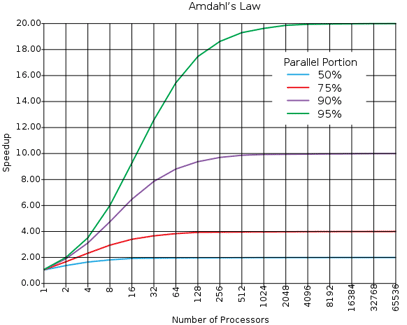
\includegraphics[width=0.7\linewidth]{amdahl}
  \vspace*{-0.3cm}
  \caption{Amdahl's Law. From \cite{noauthor_hitchhikers_nodate}}
  \label{fig: 0}
\end{figure*}

\newpage

As a result, I have chosen to use actors as my agent. I have specifically
chosen to target Erlang, since it was made for highly-concurrent, fault-tolerant
systems. Functional programming languages do not allow mutable state and thus
guarantee race freedom by design \cite{bianchi_survey_2018}.
As can be seen in figure \ref{fig: 1}, Erlang's performance is up to par with the
other languages I have explored. This will be greatly beneficial when implementing
a pool of servers within my architecture.

\begin{figure*}[ht!]
  \centering
  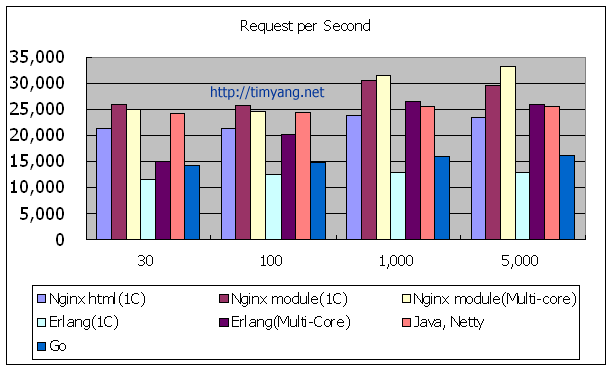
\includegraphics[width=.8\linewidth]{c_erlang_java_go}
  \caption{A graph representing the test results for web server performance in several languages. From \cite{yang_c_nodate}}
  \label{fig: 1}
\end{figure*}


\chapter{Architectural paradigms, distribution and design patterns}

Distribution is a critical consideration for highly concurrent game
environments, ensuring scalability when individual servers become
overloaded, such as during sudden traffic spikes like flash floods, as
previously mentioned {\hypersetup{linkcolor=teal}(\pageref{rationale_problem})}.
For implementing the concurrent game environments themselves, there are various architectural approaches.
To start, there is the choice between the peer-to-peer model or client-server model.
The peer-to-peer model eliminates the need for a central server, simplifying setup and
reducing costs. While this model is resilient to server failures, it presents challenges
in managing peer disconnections and potential cheating through data manipulation~\cite{franchetti_coping_2020}.
Conversely, the client-server model allows the server to act as a neutral authority to govern the game,
validating players' actions. The model does introduce more upfront challenges though, including cost,
latency, and scaling. Mitigations exist, for example, using a load balancer with multiple servers," so
that if a server goes down, another one can take its place without causing significant
disruption for clients", or by having auto-scaling so that servers "can spin up or down
based on usage" \cite{pandey_peer--peer_2022}.

\section{Pool Architectures}
%https://cubettech.com/resources/blog/microservice-v-s-pool-architecture-for-saa-s-applications/

The Pool architecture design is where every client is given a dedicated instance
of a service, executing independently inside their own separate resource pool.
This allows for individual scaling and exact resource allocation, meaning that
individual performance demands for individuals are fulfilled without other
users' interference.

Tailored scaling allows clients to adjust resources based on their unique
workload requirements, preventing unnecessary competition for resources.
Allocating resources on a per-client basis, minimizes waste and optimizes efficiency,
ensuring clients only consume what they need.
Additionally, isolation of resources inherently enhances security, as each client’s
data and services remain segregated, reducing the risk of cross-tenant
vulnerabilities.

However, having many dedicated instances introduces complexity, but there are automation
tools for deployment and monitoring to simplify things. While dedicated resources makes the model more
costly (in terms of expenses), strategic usage of resources, like dynamic provisioning, can control the costs. The
centralized nature of the resource pool also presents a single point of failure, however this may be
avoided by using robust backup mechanisms and disaster recovery protocols.

Pool architecture is particularly well-suited for B2B applications with
fluctuating traffic patterns,
where fine-grained scaling per client is critical. It is also well-suited
for enterprise environments where monolithic client programs need to have resources
assigned to them specifically, so it is easier to manage while maintaining efficiency.

While pool architecture requires careful resource allocation, it can minimize
long-term costs by eliminating over-provisioning. Because scaling is client-specific,
the financial cost of scaling a complete system is completely eliminated when just some
clients require additional capacity.

\section{Microservices}
%https://learn.microsoft.com/en-us/azure/architecture/guide/architecture-styles/microservices

Using microservices is an alternative that is fairly modern and common.
With microservices, an application is structured as a collection of small,
autonomous services with each one responsible for a specific function. This encourages decentralization
and loose coupling since each service can run separately, allowing more flexibility,
scalability, and robustness, making it well-suited for complex, dynamic systems.
This segregation makes services loosely coupled, i.e., changes to a single service need not be reflected in others.
Microservices should be independently deployable so that development teams can update,
scale, or replace a single service without disrupting the whole system. This
modularity accelerates development cycles and reduces the risk reduces the
risk involved in largescale deployments. Part of this is fault isolation; a
single service failure does not take the whole system down.
Design patterns such as the Circuit Breaker avoid cascading failures, preventing system instability.

Microservices tend to communicate with each other through APIs, enabling
services to use different programming languages, databases, and frameworks,
a concept known as polyglot persistence. For e.g., a service may use
a relational database for transactional consistency while another uses a NoSQL
database for fast read speeds. In this way,
teams can choose the best tool for the job and not be restricted by
a one-size-fits-all solution.

In order to be able to manage the complexity of distributed services, architectures using microservices
tend to have an API Gateway, a singular entry point for client requests. The gateway addresses
common concerns like authentication, load balancing, and request routing, making interactions simpler,
with enhanced security.

\phantomsection
\label{microservice_issue}

A major issue is the added operational complexity due to the decentralized
design; strong monitoring, logging, and debugging capabilities are required in
order to monitor communication between services.
Data consistency gets harder to manage as transactions can be distributed among
several services and tend to need eventual consistency rather than strict ACID
compliance. Network delay and inter-service communication overhead can impact
performance, especially in systems where there are deeply nested dependencies
between services.

Avoiding tight coupling between services, shared databases or strict
APIs, allows for long-term maintainability. Resilience patterns
such as retries and timeouts help manage failures gracefully,
and API versioning avoids compatibility issues on updates.

\addcontentsline{toc}{section}{Saga interaction}
\subsection{Saga interaction}

%https://www.infoq.com/articles/saga-orchestration-outbox/
”When moving to microservices, one of the first things to realize is that
individual services don’t exist in isolation.” As discussed
before {\hypersetup{linkcolor=teal}(\pageref{microservice_issue})}, this causes
many issues, including the major issue of maintaining data consistency across
services. One solution is the Database per Service pattern where each service
has its own database, allowing for loose coupling, independent development,
and scalability. But this adds the issue of handling transactions that span
multiple services; the Saga interaction pattern solves this issue.
%https://microservices.io/patterns/data/saga.html

A Saga is a sequence of local transactions. %https://microservices.io/patterns/data/saga.html
It makes it possible for long-running transactions to span across multiple
microservices without violating all-or-nothing semantics (either all
transactions in the sequence succeed, or the whole operation is rolled back
so that data consistency is maintained).%https://www.infoq.com/articles/saga-orchestration-outbox/

\phantomsection
\label{saga_events}
The Saga interaction pattern works by coordinating the transactions among
microservices using asynchronous messaging, likely through the use of message
brokers. Asynchronous communication is preferred since it isolates services,
i.e., failure in one service doesn't block others. %https://microservices.io/post/sagas/2019/08/04/developing-sagas-part-2.html
The microservices
broadcast an event after successfully completing a local transaction, and
the next transaction is initiated by the success or failure of the
previous one. If all transactions are successful, the operation is complete
but if any of the transactions fail, then compensating transactions are
invoked to reverse the alterations made by past transactions. %https://docs.aws.amazon.com/prescriptive-guidance/latest/modernization-data-persistence/saga-pattern.html
For example, in e-commerce, where a payment has been processed but the order
cannot be fulfilled, a compensating transaction would refund the payment.
However, designing compensating transactions can be complex as each service
must define how to reverse its changes. This complexity grows as the number
of microservices increases, making debugging and maintenance challenging.
%https://docs.aws.amazon.com/prescriptive-guidance/latest/modernization-data-persistence/saga-pattern.html

There are two main ways of implementing Saga interaction; choreography and
orchestration. In choreography, every service talks directly to the next
service in the chain. Upon completion of a local transaction, a service sends
an event that initiates the next transaction; a decentralized design that is
simple but can become difficult to work with when there are many services
as Saga logic is distributed across services, making it more difficult
to debug and comprehend.%https://www.infoq.com/articles/saga-orchestration-outbox/

In the alternative implementation, orchestration, a central ’orchestrator’
coordinates the Sagas. The orchestrator calls each service one after another
and controls the flow of messages, centralizing the logic, making it easier
to extend and maintain. For e.g., to add a new step to a Saga, you only need
to update the orchestrator, not every participating service.%https://www.infoq.com/articles/saga-orchestration-outbox/

The lack of isolation is still a large issue though, since even with the
pattern ensuring all transactions are atomic, consistent and durable
(changes are permanent), the lack of isolation means that changes from local
transactions are visible immediately, even if the Saga fails later.
%https://www.infoq.com/articles/saga-orchestration-outbox/

\section{Event driven architecture}

%https://aws.amazon.com/event-driven-architecture/

As seen in Saga interactions {\hypersetup{linkcolor=teal}(\pageref{saga_events})},
Event-Driven Architecture (EDA) and microservices are complementary. While
microservices decompose applications into independent components, EDA offers
the backbone; asynchronous communication that allows loose coupling. Although
often paired with microservices, EDA is extremely useful even in monolithic or
hybrid architectures, like Pool Architectures. EDA is widely adopted for its
scalability, flexibility, and resilience.

In EDA, events representing state changes (e.g., an e-commerce order) initiate
communication between decoupled services. Events may or may not have a data
payload, but can be used as a notification to initiate further action. The
architecture is based on three main components; event producers, routers, and
consumers. Producers and consumers are entirely decoupled so that they are
completely unaware of each other’s existence, allowing them to work
independently.

EDA's primary strengths include fault isolation (component failures don't
cascade), development agility (scalability and the lack of request-response or
polling logic), and centralized security (consistent encryption and access
control via routers). It also saves financial costs; as a push-based system,
as opposed to polling-based systems that continuously consume resources to
look for updates, processing only happens when events get emitted, avoiding
idle resource consumption and unnecessary network traffic. The router also
serves as an elastic buffer, absorbing workload spikes and providing
guaranteed event delivery, even during partial system outages.

\newpage

The pattern shines in cross-account or cross-region situations, real-time
alerting / monitoring, or concurrent processing. As an example, from one file
upload, the event router can publish an event to multiple consumers, launching
concurrent flows. It integrates heterogeneous systems seamlessly as a universal
layer of interoperability for legacy systems or polyglot services.

While EDAs offer significant advantages, their suitability depends on specific
application requirements. An EDA requires careful attention to event
permanence; if events should be processed exactly once, the source of the
event must ensure delivery and eliminate duplicates). As well as this,
tolerance of latency and out-of-order delivery, and transparency of event
flow (helping debugging) should be considered. State recovery requires
ordered, deduplicated replays of the events to avoid inconsistencies,
handling any split-brain states.

\addcontentsline{toc}{section}{Kubernetes}
\subsection{Kubernetes}

%https://enterprisersproject.com/article/2017/10/how-explain-kubernetes-plain-english
A key example of an EDA is Kubernetes.
Kubernetes is a platform that automates Linux containers. It removes most of
the manual processes involved in deploying and scaling containerized applications.
You can group (cluster) together hosts running Linux containers, and then
Kubernetes makes it simpler for you to work with the cluster. The main issue with
Kubernetes, something it's infamous for, is it's sheer complexity; "it’s a
difficult environment requiring a steep learning curve to seize its
real potential".%https://www.appvia.io/blog/why-is-kubernetes-so-complicated

%https://www.thestack.technology/playstation-gameservers-kubernetes-agones-multiplayer-games/
%https://sonyinteractive.com/en/innovation/technology/research-academia/research/fully-automated-kubernetes-operations/

Kubernetes exemplifies EDA through its reactive control loops; components like
the scheduler and controllers continuously monitor cluster state changes
(events) and reconcile actual state with desired state. This can enable
autonomous operations like scaling events and adjusting pods (the smallest
deployable units of computing). Git repositories can be watched for declarative
manifest changes, to automatically deploy updates. Even failures can become
events, like when add-ons fail, Kubernetes' self-healing mechanisms
can trigger recovery workflows.

While Kubernetes abstracts away infrastructure complexity from applications,
this comes at a steep operational price, the platform's notorious configuration
overhead. What was once application-level complexity (scaling logic, failover
mechanisms) now manifests as YAML sprawl, requiring teams to master hundreds of
parameters for networking, storage, and autoscaling just to achieve basic
functionality. This shifts the burden from developers to platform engineers,
creating a new form of vendor lock-in where simple changes require deep
Kubernetes expertise. The very decoupling that simplifies applications
paradoxically complicates the ecosystem, demanding constant tuning of the
orchestration layer that now holds all the moving parts.

Kubernetes' greatest strength, externalizing infrastructure concerns, becomes
its weakness when organizations underestimate the operational tax. By
divorcing applications from their runtime environment, Kubernetes creates a
meta-problem: now you're not just debugging your code, but debugging the
platform that runs your code. The abstraction leaks when teams spend more time
wrestling with the environment, rather than writing business logic, proving that
complexity never disappears, it just relocates.

%percentages are https://sonyinteractive.com/en/innovation/technology/research-academia/research/fully-automated-kubernetes-operations/
As mentioned {\hypersetup{linkcolor=teal}(\pageref{rationale})}, companies have
wanted to / have swapped out their architectures
for ones that better suit their need. A prime example is PlayStation running
their game servers on Kubernetes. By treating everything as an event (node failures, traffic spikes, security
patches), they transformed Kubernetes from a manually managed orchestrator
into a self-regulating platform where the system itself becomes the first
responder. They managed to cut cluster creation time by
90\%, reduce the Recovery Time Objective (RTO) (the maximum acceptable downtime
based on business requirements) by 90\% and reduced deployment times by 70\%,
a testament to the scalability, flexibility, and cost-effectiveness of Kubernetes.

\addcontentsline{toc}{section}{The Publish–Subscribe pattern}
\subsection{The Publish–Subscribe pattern}

%https://cloud.google.com/pubsub/docs/overview

Delivery patterns for events include publish/subscribe (one-to-many) and
point-to-point (one-to-one). These patterns can also be used for messaging
though messages are better suited for command execution, workflow
orchestration, and explicit coordination. While request/reply is technically
possible, it is more commonly associated with messaging patterns rather than
pure event-driven systems.

While, Kubernetes and Pub/Sub are complementary in implementing event-driven
architectures, Pub/Sub can be used standalone in EDAs, like in Pool
architectures. While Kubernetes internalizes event-driven principles through
its control loops, Pub/Sub provides a more direct messaging layer for
cross-service communication, specializing in application-level control.
Pub/sub excels in enterprise integration scenarios where loose coupling
matters more than immediate consistency. However, this decoupling comes
with tradeoffs, unlike Kubernetes' built-in reconciliation and self-healing
capabilities, Pub/Sub implementations require explicit handling of message
retries, dead-letter queues (stores of messages that the messaging system
cannot or should not deliver), and duplicate processing.

In some modern systems, a combination of both approaches is used, leveraging
Kubernetes for infrastructure automation while using Pub/Sub for event
propagation, creating a layered event-driven architecture that separates
operational concerns from domain workflows. This hybrid approach allows
organizations to benefit from Kubernetes' orchestration power while
maintaining the flexibility and scalability of asynchronous messaging for
processes.

\addcontentsline{toc}{section}{Point-to-Point Messaging}
\subsection{Point-to-Point Messaging}
%https://eda-visuals.boyney.io/visuals/point-to-point-messaging
Point-to-point messaging implements a targeted methodology in EDAs, a
lightweight alternative to Pub/Sub's broadcasting model. Its implementation
establishes direct channels between message producers and consumers, where
messages that enter are placed into queue and processed by consumers at
their own pace. This approach is effective for workload distribution as it
allows horizontal scaling through competing consumers that simultaneously
pull messages from the same queue.

When working with variable processing loads or rate-limited systems, it is
especially useful, since consumers can throttle their message consumption to
match their capacity. Unlike Pub/Sub's event broadcasting, where all
subscribers are expected to require all messages, point-to-point channels
make use of a more focused delivery mechanism, where each message is
handled exactly once, making it well suited for task distribution and
job queues.

The channel queue serves as an elastic buffer, absorbing traffic spikes while
enabling consumers to process messages at sustainable rates, preventing
overloads common in synchronous systems. In EDAs, this pattern is an
essential mechanism for situations where ordered processing, load balancing,
or integration with systems that cannot handle Pub/Sub's fire-and-forget
semantics is needed, augmenting instead of replacing more general event
distribution patterns.

\newpage

\section{Communication Technologies}

\subsection{Traditional Communication Protocols}

%https://www.ijcaonline.org/archives/volume46/number7/6920-9285/
Traditional communication protocols like TCP, though appropriate for general
data transmission, are not adequate for real-time systems that require immediate
interactions. TCP's connection-oriented approach, three-way handshake, and
guaranteed delivery mechanisms result in latencies that make TCP unsuitable
for highly concurrent architectures that require responses within milliseconds.
These protocols also preserve state for each connection, introducing
scalability issues when there are thousands of concurrent real-time events.

Similarly, though UDP's lightweight, connectionless design provides ultra-low
latency, appropriate for real-time applications, it poses significant issues in
concurrent settings where state synchronization and reliability is required.
Without built-in congestion control, ordering, or retransmission capabilities,
UDP burdens developers with implementing them manually; a complex task when
synchronizing thousands of concurrent connections. In highly concurrent
environments, unrestricted UDP traffic can lead to packet storms, dropped
updates for critical states, and unfair bandwidth allocation across
connections. The stateless nature of the protocol also complicates session
management as it requires custom solutions for authentication and flow control,
something TCP offers natively.

\subsection{Real-time Communication}

%https://ieeexplore.ieee.org/document/7160422
For real-time communication, solutions include, polling, long polling and WebSockets. In polling,
clients send requests to the server regularly, with the server responding with a new message, or
an empty response, if there isn't one. This has the obvious drawback of keeping load on the server,
and consuming network bandwidth while there are no new messages. To prevent receiving client requests
while there are no new messages, in long polling, the server does not send an empty response. Instead,
it holds the current request until a new message is available or a timeout expires. An issue still remains,
a connection still has to be kept alive and saved locally on the server.

WebSockets are a solution to both issues. "With WebSockets, we can reduce the metadata (HTTP headers) that are sent in
every request (a shortcoming of Polling) and we can also provide full–duplex communication through a
single socket (a shortcoming of Long Polling)". This would make WebSockets the choice for real-time
communication, however they are not perfect, for e.g., they are still susceptible to DoS attacks
\cite{gupta_overview_2018}. While WebSockets provide full-duplex real-time communication, they are
fundamentally built atop TCP, inheriting its reliable ordered delivery but
also its connection overhead on the initial request. This is mitigated for
future messaging as the connection is persistent after the initial
handshake, providing the benefits of TCP without most of the overhead.
The result of using WebSockets is near-real-time communication, ideal for
applications like live chats, gaming, or financial tickers that need both
reliability and sustained high-frequency messaging.

An alternative to the use of WebSockets is WebRTC. WebRTC utilizes UDP by
layering protocols on top, introducing selective reliability through SCTP
streams, allowing developers to choose between loss-tolerant media channels and
guaranteed-delivery data channels within the same session, as well as
in-order or out-of-order delivery. It is capable of
managing thousands of concurrent peers with dynamic congestion control to
prevent connection starvation in crowded networks. By
adding just enough structure to UDP without sacrificing its speed advantages,
WebRTC delivers the predictability required for scalable concurrency.
While WebRTC applies concurrency-aware constraints to UDP's wild efficiency,
WebSockets inherit TCP's concurrency limitations at the protocol level.

\section{The CAP theorem}

%https://www.splunk.com/en_us/blog/learn/cap-theorem.html
The CAP theorem is a core concept in distributed system design. It states that
in designing a distributed system, there needs to be a choice between three
properties: consistency, availability, and partition tolerance. The theorem
states that it is not possible for a system to provide all three at once,
and that careful consideration of the trade-offs is required.

For Consistency, all of the nodes in a system must have the same information
at all times. On a write occurring, all following reads must provide the latest
value, regardless of which node handles the request. This makes the data
accurate but usually adds latency and lowers availability, particularly
during network issues. Ensuring strict consistency involves coordination
amongst nodes, impacting system performance.

As for Availability, it ensures that every request has a response, even when
some nodes are unavailable. The system should continue to be operational and
responsive, but it may return slightly old results sometimes. This is
essential in systems where reliability (uptime) is more important than
accuracy of data. Methods such as data replication and load balancing
ensure availability although they can produce eventual consistency instead
of immediate consistency over all nodes.

Partition tolerance guarantees that the system keeps working when network or
communication failures occur amongst nodes. Network partitions are unavoidable
in distributed systems, so partition tolerance is generally accepted as a
requirement for designing fault-tolerant systems. Without it, any network
failure would render the entire system unavailable, which tends to be
unacceptable for most real-world applications.

% venn diagram from https://www.splunk.com/en_us/blog/learn/cap-theorem.html

Practically, system designers must compromise, choosing two properties to focus
on, like the platforms that I had surveyed {\hypersetup{linkcolor=teal}(\pageref{survey})}.
CP systems assure data correctness even in network partitions but
can sacrifice availability. They are representative of financial systems
where data consistency is of paramount importance. AP systems operate even
during failures, but at the expense of returning slightly old data. They
are best used in applications like social networking sites where
responsiveness is what matters most. CA systems are not common in the
real world, as they expect ideal networks which don't reflect
real-world conditions.

Modern distributed systems often implement a flexible approach that can modify
behavior based on current conditions. The majority of databases allow
configuration between consistency models, sometimes with a compromise being
offered between them. These trade-offs can assist architects in designing
systems tailored to their specific requirements without sacrificing
reliability and performance.

\section{My choices for distribution, architecture and system design}

After evaluating the various distributed system patterns,
I determined that a load-balanced server pool best fits my architectural
needs. To start, I chose a client-server model for easier error handling,
especially when handling peer disconnections.Between Microservice and Pool
architecture, no tool is superior to the other
since they both have varying use cases.%https://cubettech.com/resources/blog/microservice-v-s-pool-architecture-for-saa-s-applications/

Since I chose to use the actor concurrency model implemented by the OTP
framework, I would already have complete process isolation, fault tolerance,
and distributed computing capabilities at the language level, making
the adoption of microservices redundant, introducing unnecessary complexity
and overhead without providing significant additional benefits.
Using actors can be seen to be like 'microservices within a single VM', while
avoiding the network latency, deployment complexity, and interservice
communication challenges.

%https://www.appvia.io/blog/why-is-kubernetes-so-complicated
As Kubernetes is infamously complex, although it makes the application easier
to write, it would be infeasible to use as I have already chosen to learn a
lot of new technologies. As a result, I adopted a pool architecture which
provides the necessary scalability without introducing unnecessary complexity.

This approach is nice as it was a widely adopted solution for example
services I found during my research (namely the ones here; %https://medium.com/@dragonblade9x/making-a-multiplayer-web-game-with-websocket-that-can-be-scalable-to-millions-of-users-923cc8bd4d3b
)%https://jofranchetti.medium.com/coping-with-quarantine-by-coding-597372a17746
, providing
well-documented reference material, community support and troubleshooting
resources.
Given the BEAM's capabilities, a Kubernetes-based system could be excessive
for the project’s requirements, as a simple server pool can provide
sufficient scalability for the current scope (which does not include
large-scale deployment). If the scale did need to increase, the
codebase can be adapted for Kubernetes, as the app’s modular design
ensures flexibility, allowing for straightforward addition and removal of
dependencies for the transition to Kubernetes.

I chose to use the Pub/Sub pattern over point-to-point messaging due to
its inherent support for decoupled one-to-many event distribution, which
better aligns with the scalability and flexibility requirements,
especially since the servers must react to the same events asynchronously,
in real-time and without any coordination. I also chose to use WebSockets over
WebRTC because I need reliable, ordered message
delivery with simpler infrastructure, avoiding unnecessary complexity and
media-focused protocols, when all I require is robust real-time data
transfer through standard web technology.

I will mostly focus on availability and partition tolerance, while trying to
maintain consistency as much as possible,
mitigating all forseeable risks (like those mentioned here; {\hypersetup{linkcolor=teal}(\pageref{rationale_problem})}) via the use of
a load balancers, Pub/Sub, etc.. The use of my architecture, specific to
the different prototypes and applications, will be further discussed within the
description of implementations section of this report.

\chapter{Software Engineering}

\section{Methodology}
Employing an engineering approach is crucial in system development. I began with
requirement analysis to capture functional needs, leading to detailed use case
descriptions and a comprehensive use case diagram. This foundation allowed me to
create UML sequence diagrams that map out system interactions. Throughout development,
version control enabled me to experiment with new features or fixes without
affecting the main codebase, while a solid test strategy identified and resolved
defects early, ensuring the system's reliability and performance.

\begin{figure*}[ht!]
  \centering
  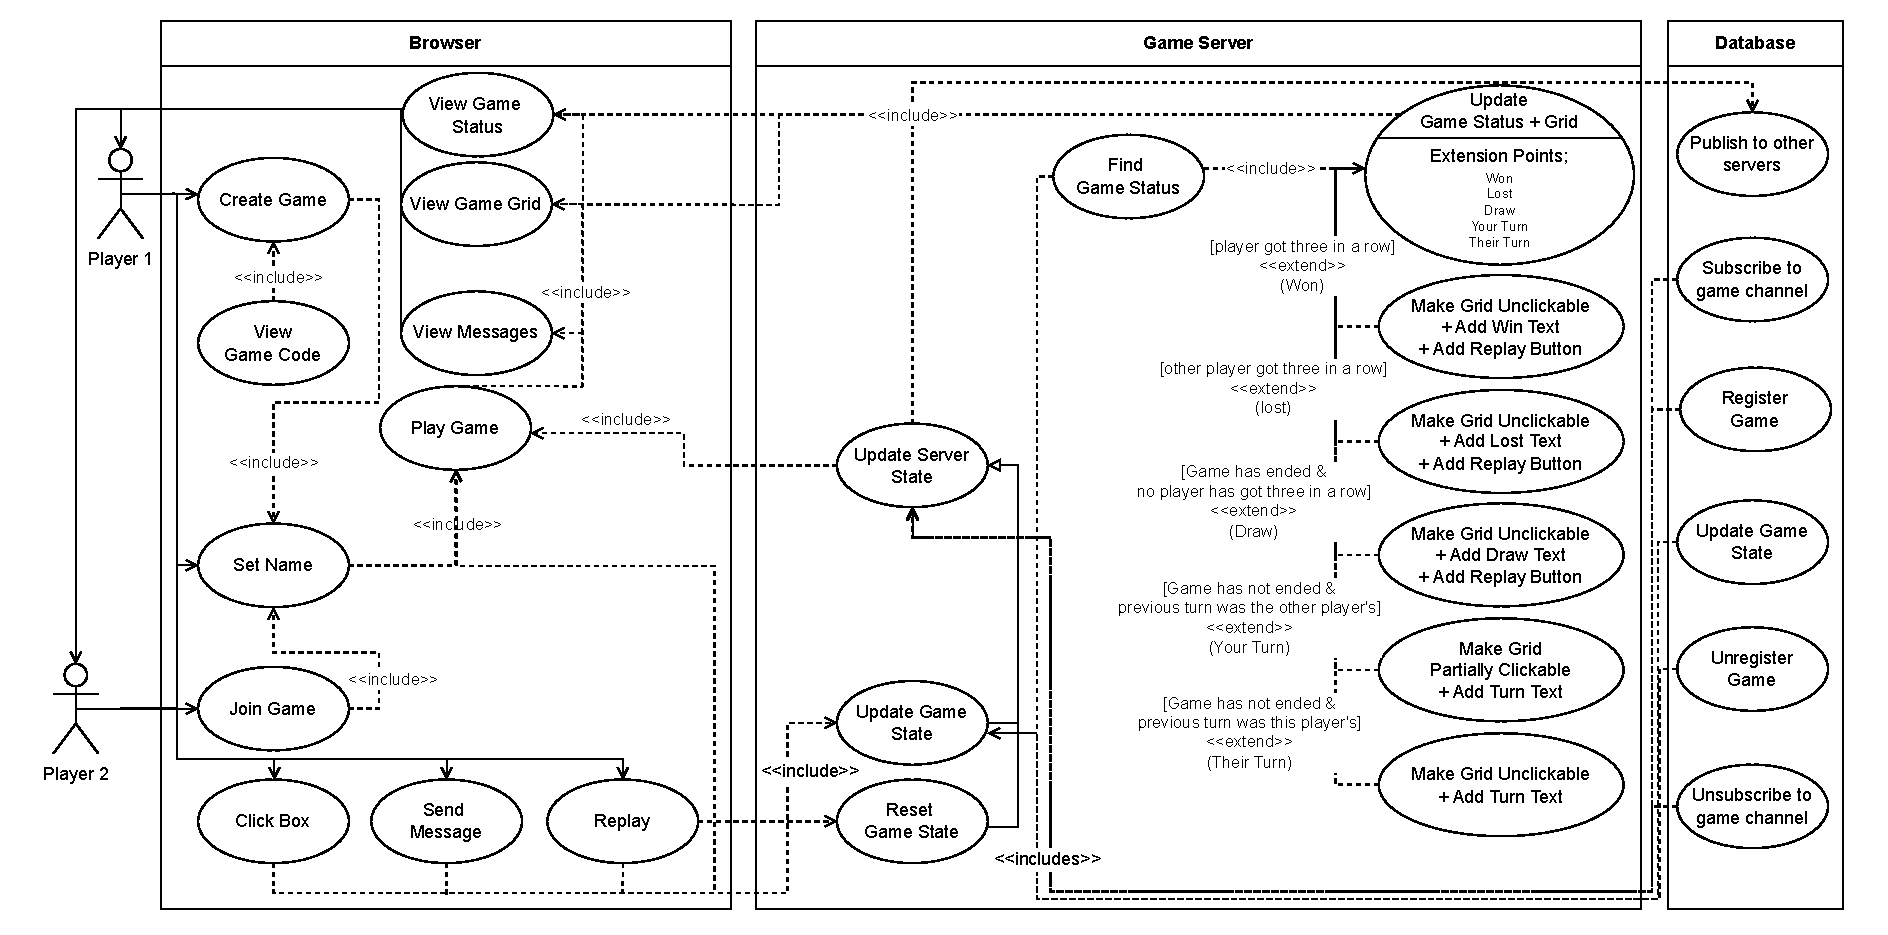
\includegraphics[width=\linewidth]{use_case}
  \vspace*{-0.5cm}
  \caption{A use-case diagram for the Tic-Tac-Toe game}
  \label{fig: 2}
\end{figure*}

In my project, I did not create a class diagram due to the use of the functional
programming paradigm. Instead, I focused on use case diagrams and sequence diagrams,
as detailed further below. In functional programming, it is more common to begin
by writing the signatures of the top-level functions. As more detail is needed,
signatures for helper functions are subsequently defined \cite{Wlaschin_functional_2014}.
This was done alongside writing the types that the function signatures use. "Type design and function
signature design are really two faces of the same coin."\cite{noauthor_chapter_2024}
This approach is effective because functional programming lacks side effects; functions are
specified solely in terms of their inputs and outputs. Consequently,
type signatures serve as a powerful design tool, providing clarity and structure.
This contrasts with imperative programming, where side effects often complicate
the design process. Despite the compiler's ability to infer type signatures,
they are explicitly used to enhance readability and maintainability of the code.

I also tried to use design patterns, a set of software engineering
techniques which aim to address recurring issues within development. Some of these
issues are reducing the complexity of code, increasing the cohesiveness of code,
and improving reusability. I particularly aimed to use functional patterns, including
writing endomorphisms, monoids which are functions that use the same type for their
input and output\cite{Wlaschin_functional_2014}, as well as using monadic binds
wherever possible, to make my code linear and clear. While this is visible
throughout the codebase, as this was my first time doing functional programming,
I suspect there are many more design patterns and refactoring opportunities to explore
to enhance the codebase.

To ensure a robust and reliable development process, I utilized a private GitHub repository
alongside the departmentally mandated GitLab instance. This approach not only mitigated
the risk of data loss due to hardware failure but also leveraged the many benefits of
version control. By consistently committing and pushing work, following a consistent
git workflow, branching model and naming schemes, I was able to track changes
over time, providing a detailed history of the project's evolution. This made
it easier to identify and revert to previous versions when necessary. Version
control also facilitated branching and merging, allowing me to experiment with
new features or fixes without affecting the main codebase. This maintained a
clear record of progress and decisions, invaluable for documentation and debugging.
These capabilities ensured a more organized, efficient, and resilient development
process, enhancing the overall quality and reliability of the project.

\section{Testing}
Testing is an essential component of software development. Tests can be used to
help identify bugs within code early on, and can also aid in the debugging process.
Most games don't follow TDD; in game development, play-testing is commonly favored
over unit testing due to the need to assess visual elements like animations and
latency in real-time.\cite{politowski_survey_2021} TDD requires developers to know
in advance what they want to
achieve so they can write tests before creating the functions. Game developers often don't
have this complete knowledge initially, leading to tests that fail even when the function
works as intended. This makes TDD challenging in game development, as developers may
need to rewrite tests later, defeating the purpose of the technique.

In my project, I only wrote unit tests for functions without server
dependencies, relying on end-to-end testing for those requiring server interaction.
Even though my unit tests are few(er) in number, I have still tested all code through
end to end testing, including browser automation tests via chrobot, a package providing
an interface and bindings to the Chrome Devtools Protocol \cite{noauthor_chrobot_nodate},
and informal play testing.

\section{Documentation}
Gleam's comprehensive, built-in tooling significantly streamlined development by
providing code formatting, type-checking, formatting, refactoring actions, documentation support, etc.,
ensuring consistent code quality while minimizing manual configuration, and
options that can lead to inconsistencies between codebases, hurting code
readability.

It helped generating web pages to display the documentation (similar to JavaDoc)
for public types and functions, helping the development process.
I documented all modules, types, and functions, including private ones,
in order to enhance code reuse and adaptation. This thorough approach not
only simplifies future maintenance and optimizations but also helps facilitate a
deeper understanding of the codebase.
Having comprehensive documentation
ensures that any possible future modifications or enhancements can be made
efficiently, maintaining a high standard of code quality and usability.

In solo projects, documenting code is especially beneficial, even if the advantages
aren't immediately apparent. Since the project is developed over an extended period
and includes many unique modules and functions, after a significant break from a
feature, it can be challenging to recall the purpose of each module or function.
This leads to backtracking to understand the rationale behind old code.
Comprehensive documentation helps quick identification of why specific decisions
were made and the intent behind certain pieces of code.

\chapter{A Description of the Prototype Implementations}

Developing prototypes was crucial for validating the architectural design,
testing concurrency mechanisms, and iteratively refining the game environment's
core technologies and interaction patterns before working on the final,
more complex game. With the exception of JavaScript,
all technologies in the tech stack were new to me, which led to
significant learning and growth.

This section will focus on the Tic-Tac-Toe prototype targeting Erlang,
as the JavaScript prototypes were primarily exploratory tools for learning
new technologies like WebSockets, Valkey, Gleam and functional programming.
The other Erlang prototypes share a similar, modular implementation,
optimized for the final game. The online chat's functionality is
encapsulated within the Tic-Tac-Toe prototype, and the Pong game
served to demonstrate the versatility of the underlying game
environment architecture. (Since the Pong prototype was made only for this purpose,
I modified an implementation of the game from GeeksforGeeks, to demonstrate this).\cite{GeeksforGeeks_pong_2021}

\section{Architecture}

\begin{figure*}[ht!]
  \centering
  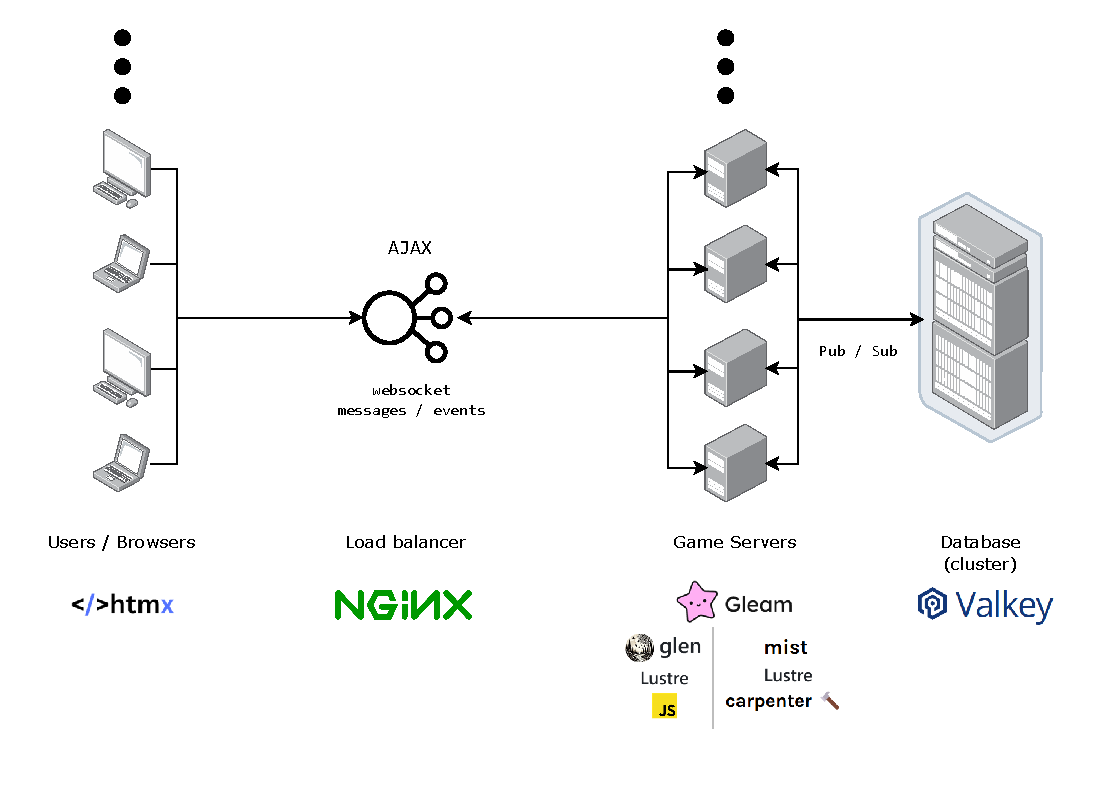
\includegraphics[width=\linewidth]{architecture}
  \vspace*{-1.5cm}
  \caption{A diagram representing the game environment architecture I chose to use}
  \label{fig: 3}
\end{figure*}

\newpage

The client-side is managed by the HTMX library, as the main focus for my project
was on the architecture of the environment and the implementation of the game
servers. The simplicity and power of HTMX, giving me access to AJAX, CSS Transitions,
WebSockets and Server Sent Events, directly in HTML through attributes,\cite{noauthor_HTMX_nodate} allowed me to
focus on the server, as I tried to make the client-side stateless. I mostly
used the WebSockets extension for the library. It had many useful features;
"if the WebSocket is closed unexpectedly, due to \lstinline|Abnormal Closure|, \lstinline|Service Restart|
or \lstinline|Try Again Later|, the extension will attempt to reconnect until the connection
is reestablished. [...] The extension also implements a simple queuing mechanism that
keeps messages in memory when the socket is not in \lstinline|OPEN| state and sends
them once the connection is restored."\cite{noauthor_HTMX_ws_nodate} Other useful features include the
use of a full-jitter exponential-backoff algorithm that chooses a randomized
retry delay that grows exponentially over time, and the exposed
set of events that allow you to observe and customize the extensions behavior
\cite{noauthor_HTMX_ws_nodate}.

This exposed set of events was especially useful in the Pong prototype as
it had a unique approach to including data to the WebSocket message; it used
a hidden field to save local data. Since the game was adapted from
client-side JavaScript, I was able to use event handlers to add data to the
hidden field whenever a JavaScript state value was modified, and trigger
sending a WebSocket message with the contents of the field.

To avoid issues like the previously mentioned ones the CodinGame platform
experienced {\hypersetup{linkcolor=teal}(\pageref{rationale_problem})}, I
implemented one of the
solutions to their problem, which was the use of a load balancer and a pool
of servers\cite{jobert_story_2017}. The load balancer uses nginx, which can
support more requests
than the game servers that are running the Erlang code (compiled Gleam code),
as seen in figure 3.2, allowing it to keep up with influxes of users.
The load balancer ensures that servers do not have their buffers overfilled
and that load is distributed evenly so that the game service can operate smoothly.
As well as this, it allows for easier scalability, as all that needs to be managed is the
number of servers in the pool.

%TODO fix links to figures

The game servers themselves were written in Gleam, with the JavaScript prototypes
using glen as their web framework, lustre for their components and HTML templates,
and some JavaScript through a FFI, to manage local state. For the prototypes
targeting Erlang, mist was used as the web server, due to it's mature state
and support for WebSockets, and carpenter for access to ETS tables, for managing
local state. Since Gleam compiles to Erlang, I could build a fault-tolerant
system, due to certain notions like 'Shared Nothing' and the lack for a need
of locks. Lustre was used solely as a component framework due to it's web server model
not being able to handle more than one socket at an endpoint at the same time.
I had also considered using wisp but it's current state, while it has matured, still
does not have good support for WebSockets as the GitHub pull request for this indicates
that the implementation makes Wisp couple too tightly to Mist \cite{noauthor_WebSockets_nodate}.

\phantomsection
\label{valkeyRead}

Valkey was used as the database since it is a fork of Redis OSS.
This means that it can scale horizontally as a Cluster, resulting in
the ability to "automatically split the dataset among multiple nodes", and
"continue operations when a subset of the nodes are experiencing failures
or are unable to communicate with the rest of the cluster"\cite{noauthor_scale_nodate}.
This ensures scalability and some tolerance towards hardware failure and data loss.
As well as this, Redis focuses on consistency and partition tolerance, as other nodes
can be spun up if availability starts to become an issue; when compared with
MongoDB, and Cassandra, Redis had the best read performance. This is due to the fact that data is stored and retrieved using
volatile memory \cite{department_of_information_systems_university_of_nizwa_sultanate_of_oman_study_2022}.

\phantomsection
\label{valkeyMessageBroker}

I mostly used Valkey as a message broker, within the Pub/Sub model, as I
tried to keep state on the game servers themselves, reducing the risk of data
loss, as all servers try to maintain the same state through sending messages
via Pub/Sub. The Pub/Sub pattern is a vital part of this architecture as it
allows all of the servers to update each other on actions being carried out
in the game, allowing all of them to maintain the same state,
instead of being inconsistent. In the Online Chat prototype,
I did save messages in the database, so that users who joined
a chat room later than the creator, could still see old messages, and so that all
users could disconnect from a chat room, and join back in and still see the old
messages.

\newpage

\section{Code implementation}

The subsequent sequence diagrams would also include a subscriber actor
but it is not included since it does not do much on the same server
messages are being published from, other than disregard the message.
Other servers would have a subscriber actor too and use it to update
their other actors' states in accordance with what updated in the game,
denoted by the published message.

\addcontentsline{toc}{section}{Client connections}
\subsection{Client connections}

\noindent
\begin{minipage}[t]{18em}
  \vspace*{-6cm}

  To start, figure \ref{fig: 5} demonstrates how the player will connect to the game.
  When the player enters the URL of the game's site in their browser, this sends a HTTP
  \lstinline|GET| request to the game server. The server will respond with the homepage which
  includes a HTML DIV element with the ID \lstinline|app|. This element uses the HTMX WebSockets
  extension to establish a WebSocket with the game server. This WebSocket will be
  used for all further interactions with the game server. Every WebSocket will have a corresponding
  actor on the game server they are connected to, for handling client-side messages and
  server-side events.
\end{minipage}
\hfill
\begin{minipage}[t]{20em}
  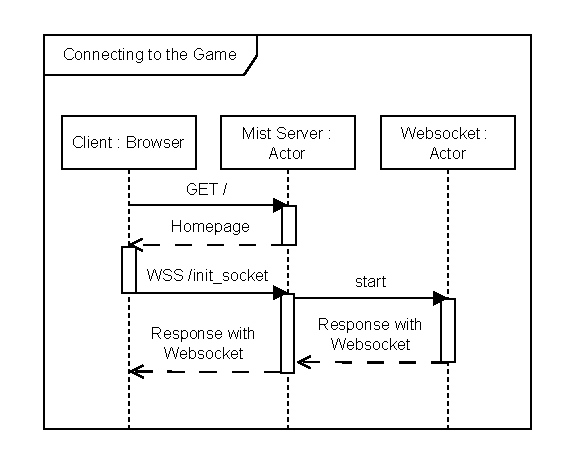
\includegraphics[width=\textwidth]{sequence_connecting}
  \captionof{figure}{A sequence diagram used for designing how the player will connect to the game}\label{fig: 5}
\end{minipage}

\newpage

\noindent
\begin{minipage}[t]{15em}
  \vspace*{-12cm}
  The code shown in figure \ref{fig: 6}, defines an \lstinline|on_init| function for the WebSocket actor. This function,
  creates a subject for the actor so that other actors can send messages to it.
  It then creates the initial state for the actor, using empty defaults where appropriate,
  as many state values will be updated over time, as the player continues towards
  joining and playing a game. Furthermore, it defines the \lstinline|on_close| function,
  which is triggered when the WebSocket disconnects, and the actor is about to shutdown. This function carries out
  'clean-up' for the different actors' states, by first checking if the player
  connected via the closed WebSocket was in a game or not and then sending the
  appropriate messages to the other actors.
\end{minipage}
\hfill
\begin{minipage}[t]{25em}
  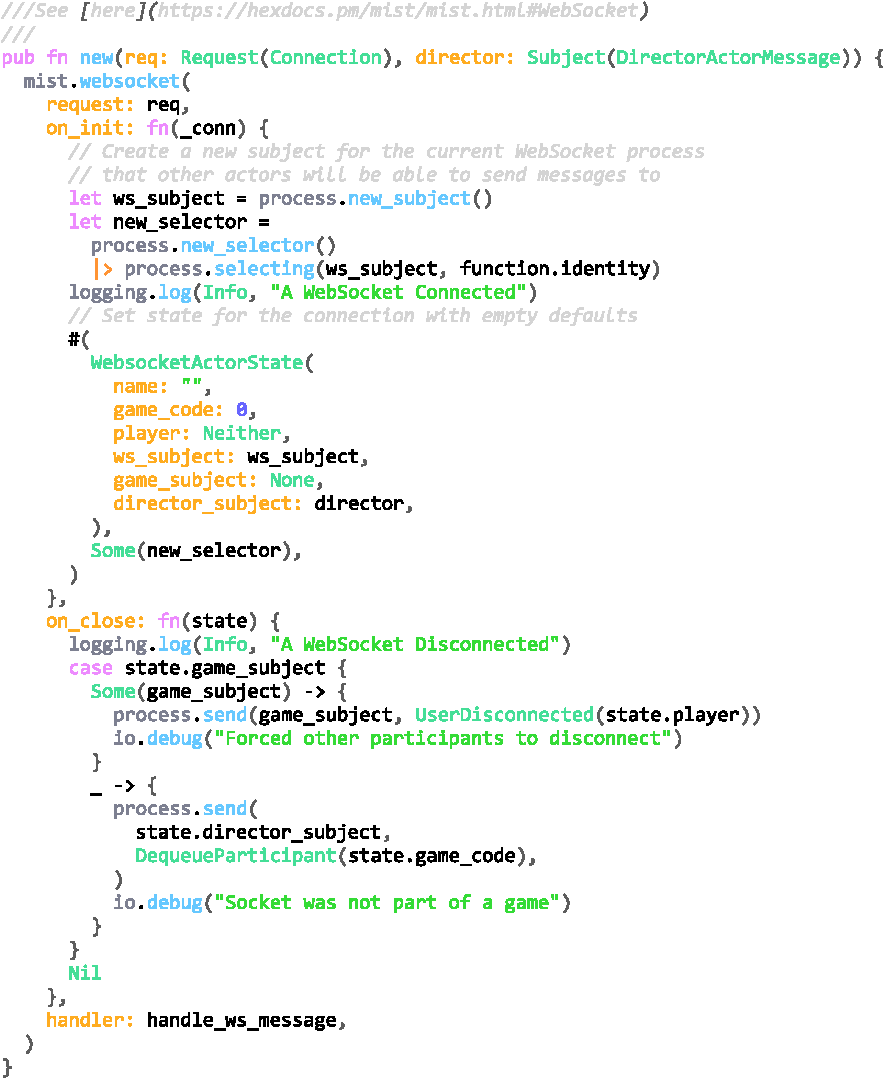
\includegraphics[width=\textwidth]{mist_websocket.pdf}
  \captionof{figure}{The function that creates the WebSocket actor and the response containing the WebSocket for the client}\label{fig:6}
\end{minipage}

\newpage

If the game actor recieves a \lstinline|UserDiconnected|
message, it will send a message to the other player's client, that will force it to disconnect
from the game after displaying the error message \lstinline|"Your opponent disconnected!"|.
Since the director actor is mostly used for managing players that are waiting for
their game to be joined, when it receives a \lstinline|DequeueParticipant| message, all it needs
to do is update its state and notify the other game servers by publishing a message.

\begin{figure*}[ht!]
  \centering
  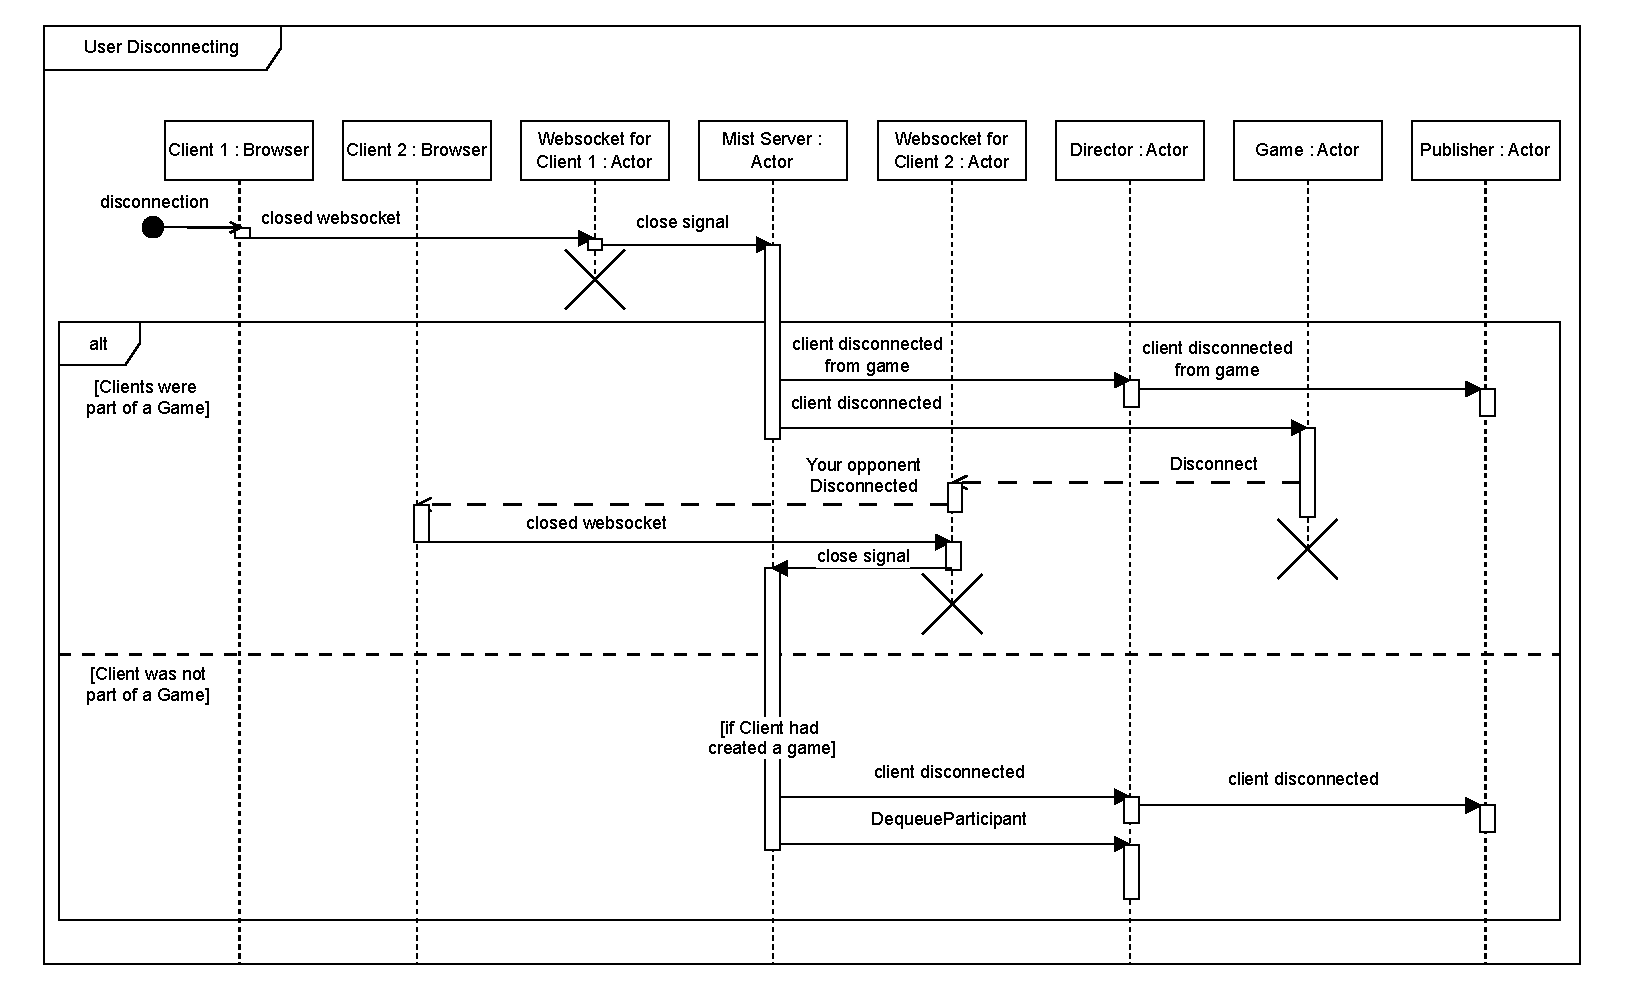
\includegraphics[width=\linewidth]{sequence_disconnecting}
  \caption{A sequence diagram used for designing how the player disconnections will be managed}
  \label{fig: 3}
\end{figure*}

\newpage
\addcontentsline{toc}{section}{Creating a game}
\subsection{Creating a game}

\begin{figure*}[ht!]
  \centering
  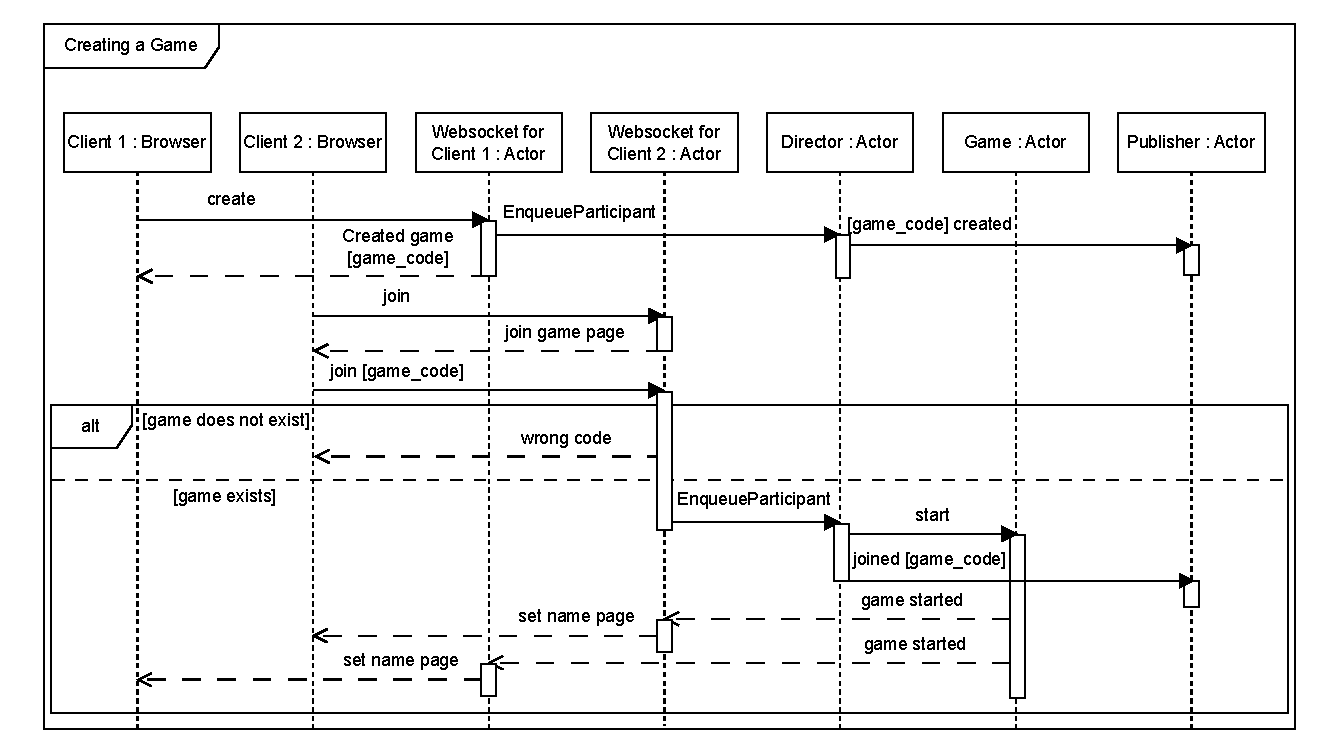
\includegraphics[width=\linewidth]{sequence_creating}
  \caption{A sequence diagram used for designing how games (rooms / sessions) will be created}
  \label{fig: 3}
\end{figure*}

When a user wishes to create a game, a stringified JSON message is sent to the game server.
This goes for any WebSocket messages to the server from the player interactions.
The message is parsed to identify that the player wishes to create a game. As seen in the diagram,
messages are sent to update the states of multiple actors, and the player's page is updated to tell
them that the game has been created, and which code to use for someone else to join it.
(The 'page' is a HTML DIV element, with the ID \lstinline|page|, within the \lstinline|app| DIV, so that the WebSocket
connection stays open). Then when a player joins the game, the director will start
a game actor for use in any further actions in that game (room / session). For simplicity,
the creator of the game is always player \lstinline|X|, and the player who joins the game is always player O.
%TODO fix single quotes too
\begin{minipage}[t]{18em}

  The director actor's state is a dictionary of 'waiting games',
  games with a single player. An ETS table is also used for keeping
  state of all games. When the player joins a game, it gets dropped
  from the dictionary, but not from the ETS table. Only when a player
  disconnects, does it get dropped from the ETS table.

\end{minipage}
\hfill
\begin{minipage}[t]{20em}
  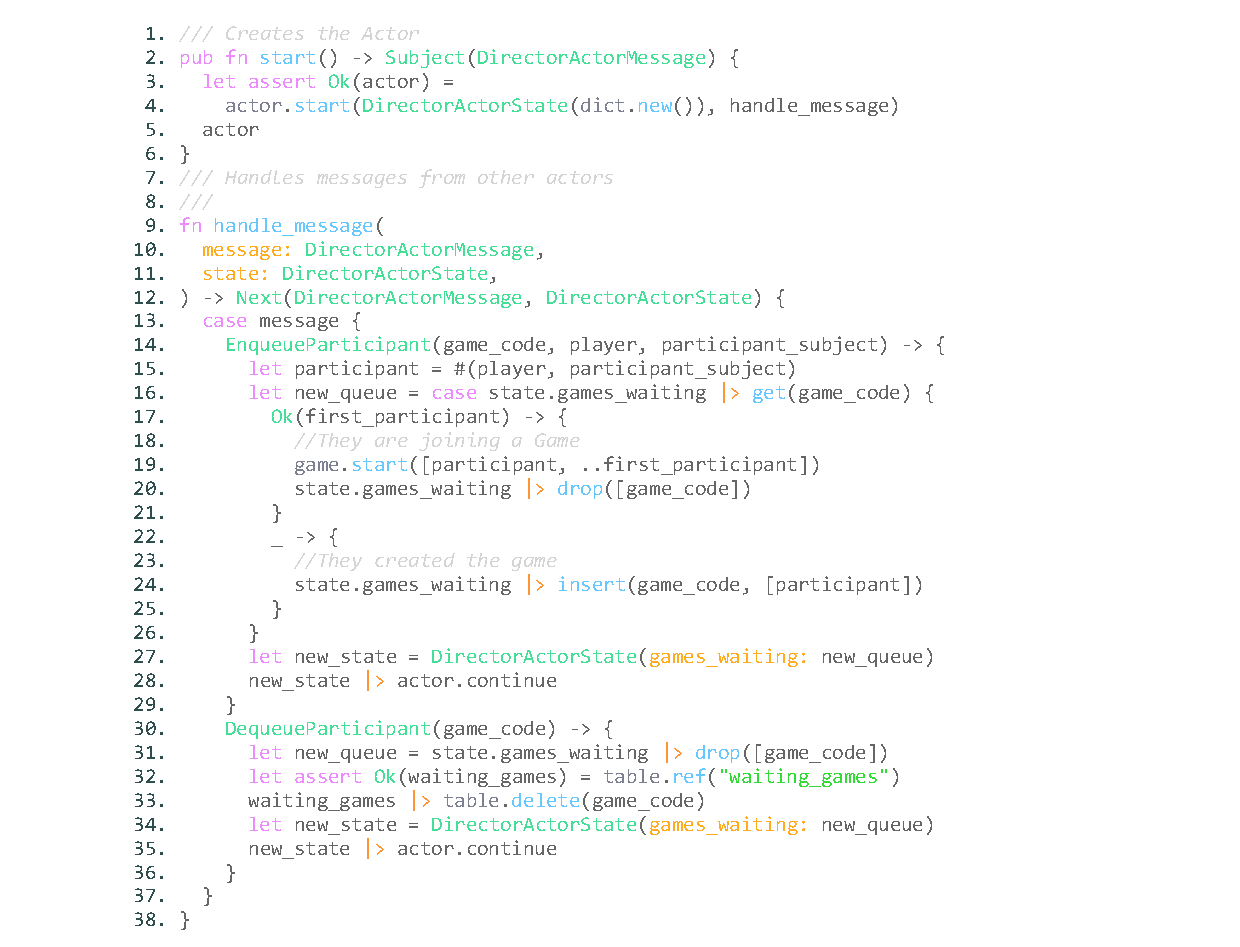
\includegraphics[width=\textwidth]{director_actor.pdf}
  \captionof{figure}{The director actor module}\label{fig: 6}
  % \vspace*{0.5cm}
\end{minipage}

\newpage

\begin{minipage}[t]{18em}
  The state of the game actor, as shown in figure 5.7
  holds the game state, using a list for the state of the Tic-Tac-Toe boxes
  where the index of the items correspond to the boxes on the page, from
  left-to-right, top-to-bottom. The initial state holds \lstinline|Neither| in
  all spaces in the list, indicating that neither player has placed
  their mark in those boxes yet.

  \vspace*{10em}

  The function in figure \ref{fig: 8} creates a random integer for the game code,
  and adds it to the ETS table as a global state for the server. This should be
  published to other servers so that their global state is synchronized. If the
  code already exists in the table, a new one is generated for the new game.
\end{minipage}
\hfill
\begin{minipage}[t]{20em}
  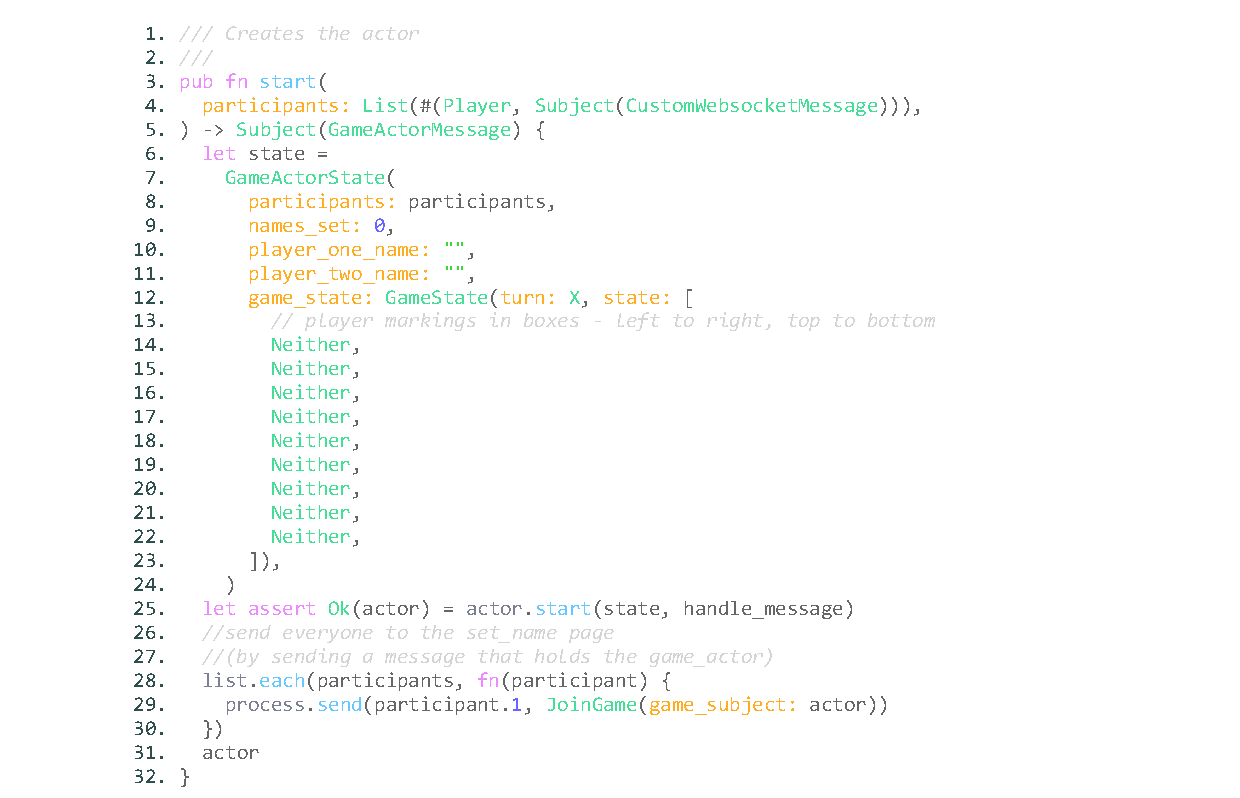
\includegraphics[width=\textwidth]{game_actor_start.pdf}
  \captionof{figure}{The function that starts the game actor}\label{fig: 7}
  \vspace*{1.5cm}
  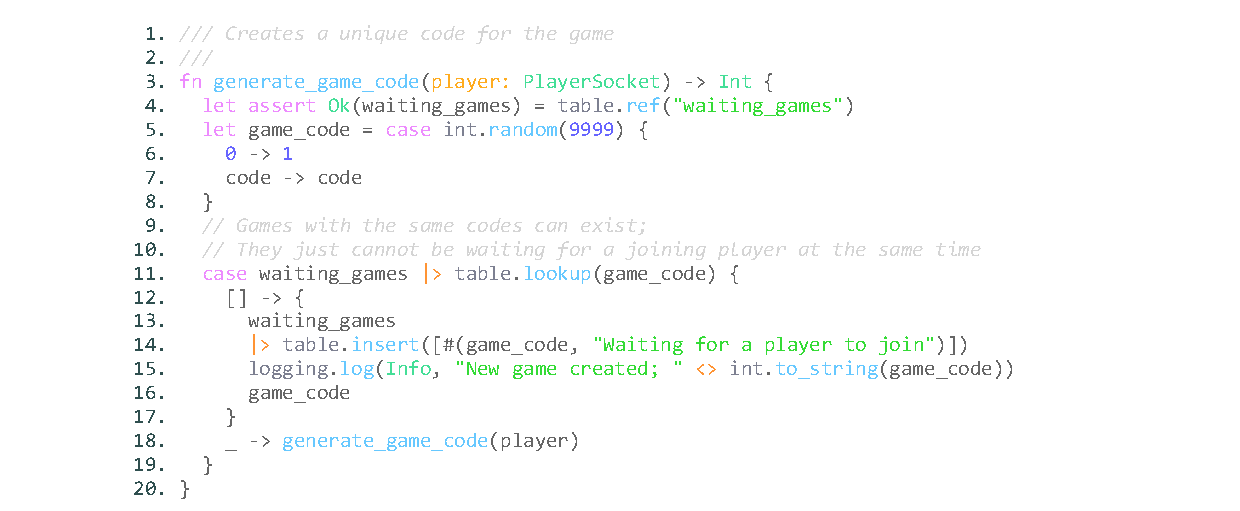
\includegraphics[width=\textwidth]{game_code_gen.pdf}
  \captionof{figure}{The function that creates a unique game code for a new game}\label{fig: 8}
\end{minipage}

\newpage

\begin{minipage}[t]{18em}
  The function in figure 5.9 decodes the message sent from the client to
  get the game code for the game they wish to join. It then checks if this game
  exists; if it does not, an error message is sent to the player, but if it does,
  a message is sent to the director actor so that it can start a game actor for the game,
  and send the players to the page where they set their name.
\end{minipage}
\hfill
\begin{minipage}[t]{20em}
  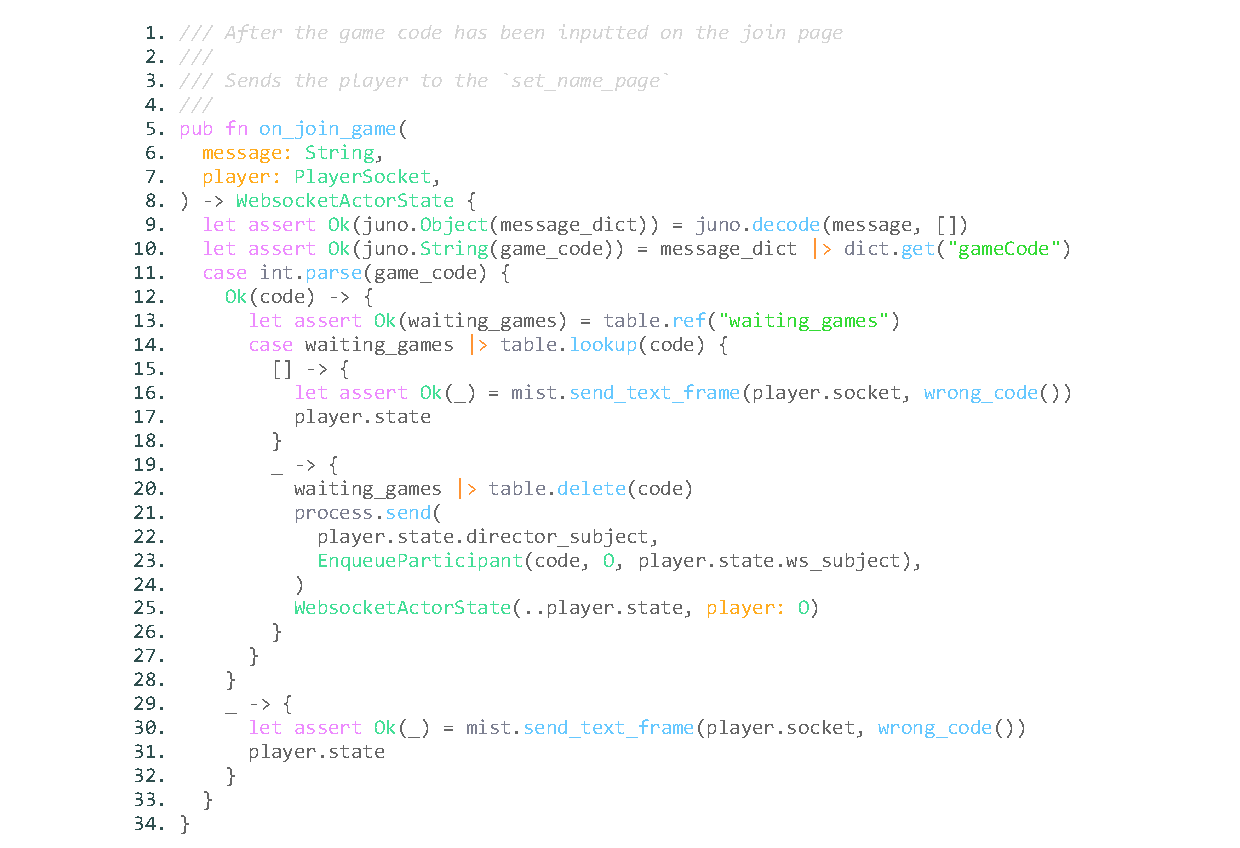
\includegraphics[width=\textwidth]{on_join_game.pdf}
  \captionof{figure}{The function to make a player join a game}\label{fig: 9}
\end{minipage}

\newpage
\addcontentsline{toc}{section}{Playing the game}
\subsection{Playing the game}

\begin{figure*}[ht!]
  \centering
  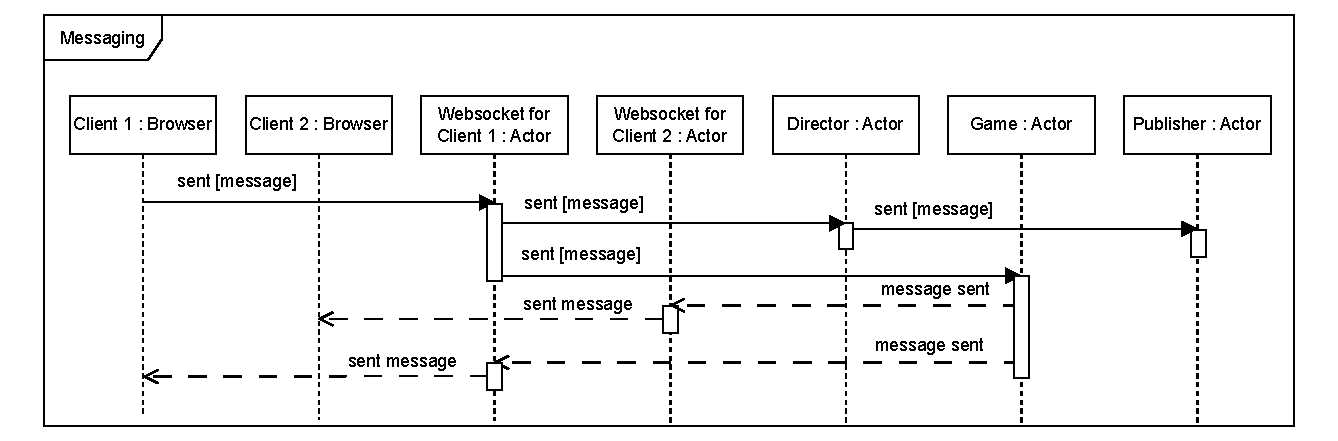
\includegraphics[width=0.9\linewidth]{sequence_messaging}
  \caption{A sequence diagram used for designing how messages within the chat will be sent}
  \label{fig: 10}
\end{figure*}

When a player sends a message in the chat, the client will send the message to
the server through their WebSocket as normal. The WebSocket actor will ask the
director actor to publish this in case the other player is connected by a WebSocket
to a different server. The WebSocket actor will also send the message to the game
actor, in case the opponent is on the same server. If so, the game actor will
send the message to the opponent's WebSocket actor so that the message can reach
the client. (The messages from the WebSocket actors to the Browsers are
stringified HTML to display with HTMX in the chat. To keep things simple, the game
actor asks both of the WebSocket actors to send this message, instead of having
the WebSocket actor of the sender, send the message first, resulting in the game
actor only needing to send the message to the opponent)

\newpage

\begin{figure*}[ht!]
  \centering
  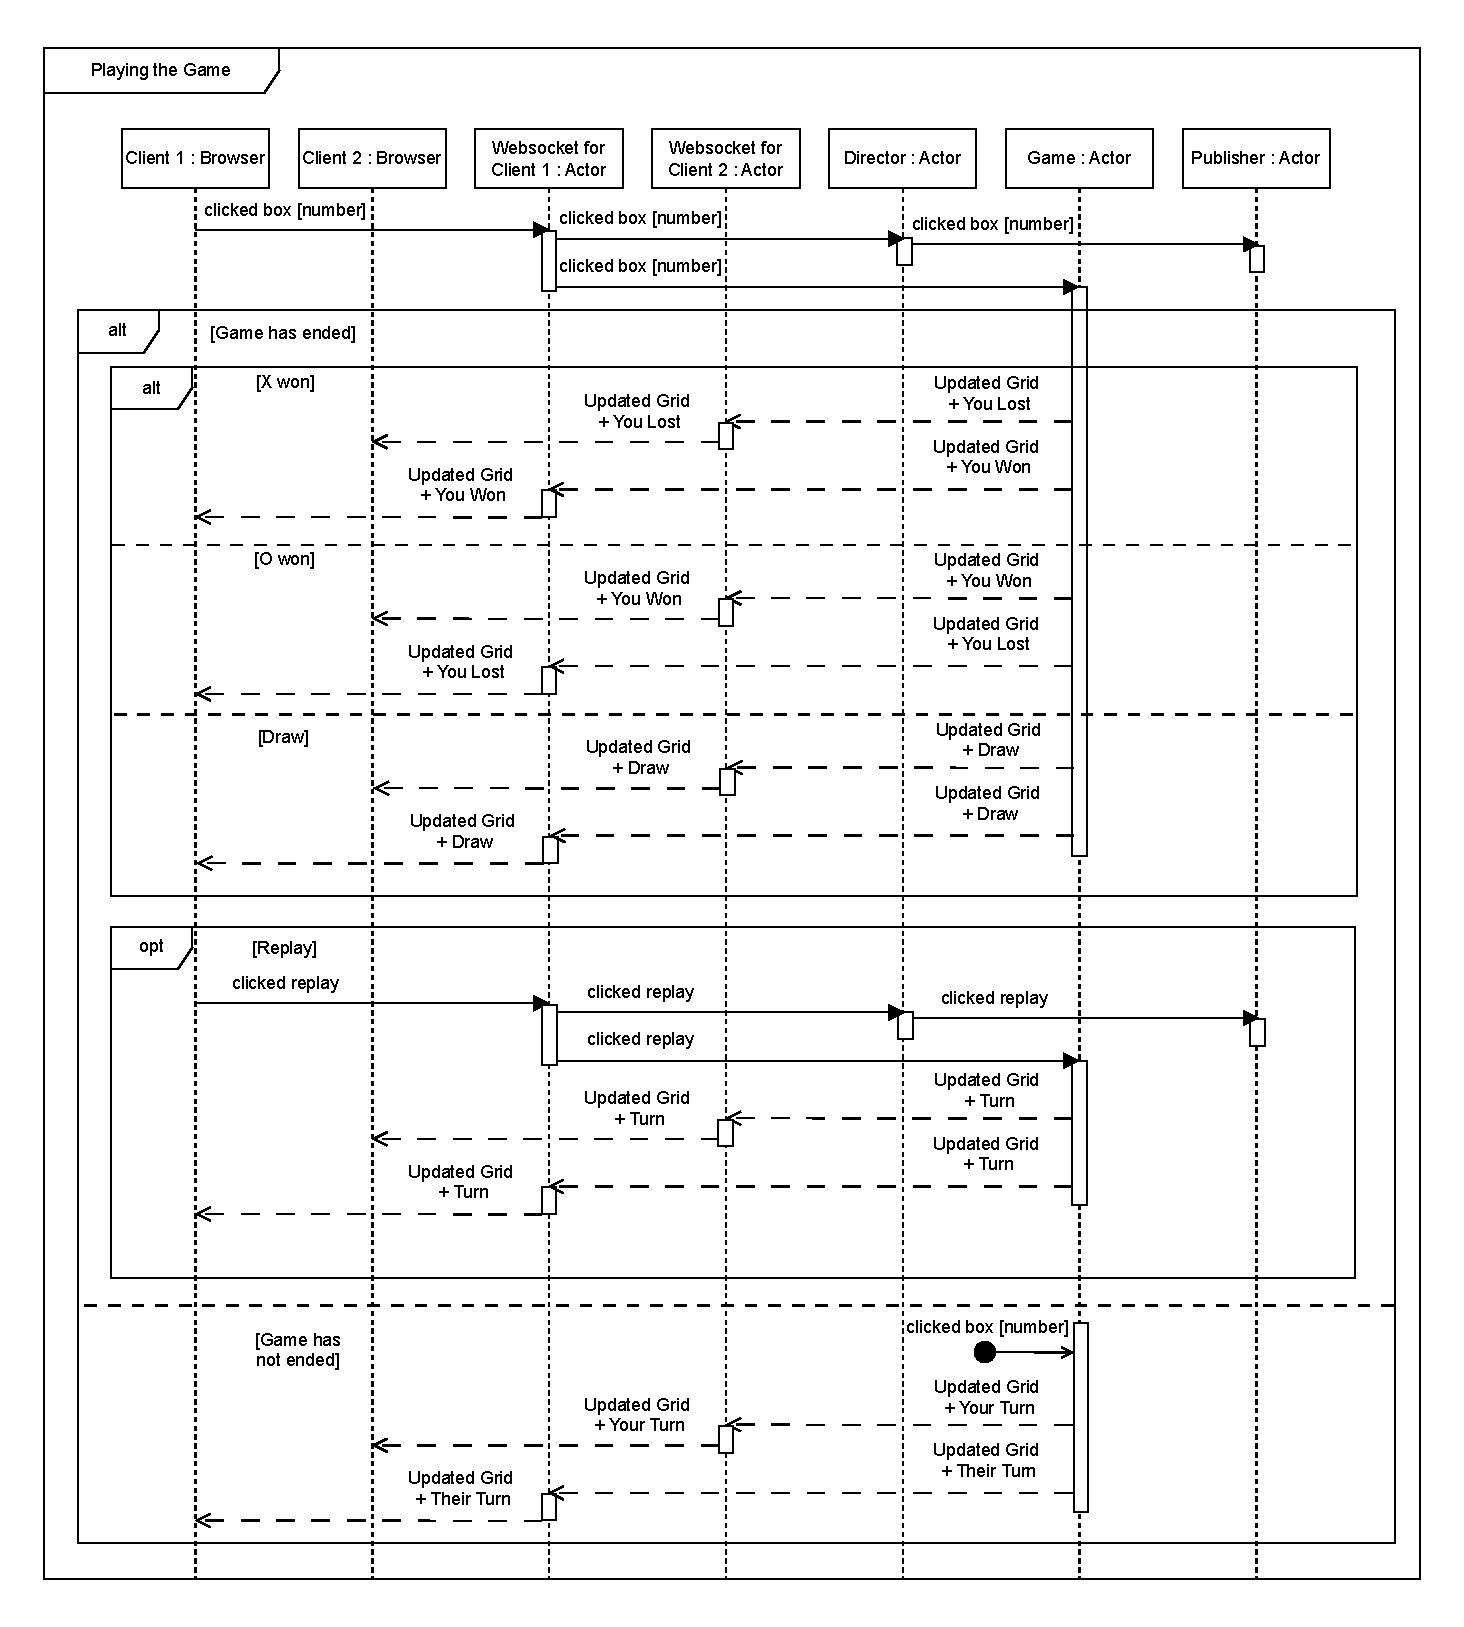
\includegraphics[width=\linewidth]{sequence_playing}
  \caption{A sequence diagram used for designing how the game will be played (Assuming Client 1 is player X, and Client 2 is player O)}
  \label{fig: 11}
\end{figure*}

To play the game, the player whose turn it is will click on a box on the game board
(The opponent will not be able to). This is published to other servers in case the
opponent is not connected to the same server. The game actor checks if the game
has ended, by checking if all spaces / boxes on the grid have been marked by a player.
If so, both players get told whether they have won or lost the game or if it was a draw,
allowing them to hit replay in case they wish to play again. If they do hit replay,
the game state is reset and the player who did not take the first turn last time
will get to go first this time. If the game has not ended after the marking of a box,
the grids for both players will be updated, as well as the game status (whose turn it is),
allowing the opponent to take their turn.

\newpage

\begin{minipage}[t]{18em}

  The code in figure \ref{fig: 9} is from the message handler in the game actor.
  When a box is clicked, the game actor's game state is updated with the new
  grid marking and next player turn. The winner is obtained from the code in
  figure \ref{fig: 10}, and is used in determining the HTML to send to the client.
  If the game has ended, or it is not the player's turn, the game grid will not be
  clickable (HTML created by \lstinline|game.game_grid|). The status text is also
  updated with \lstinline|"Your Turn"|, \lstinline|"Their Turn"|, \lstinline|"You Won"|,
  \lstinline|"You Lost"| or \lstinline|"Draw"| (HTML created by \lstinline|game.update_status|).

\end{minipage}
\hfill
\begin{minipage}[t]{20em}
  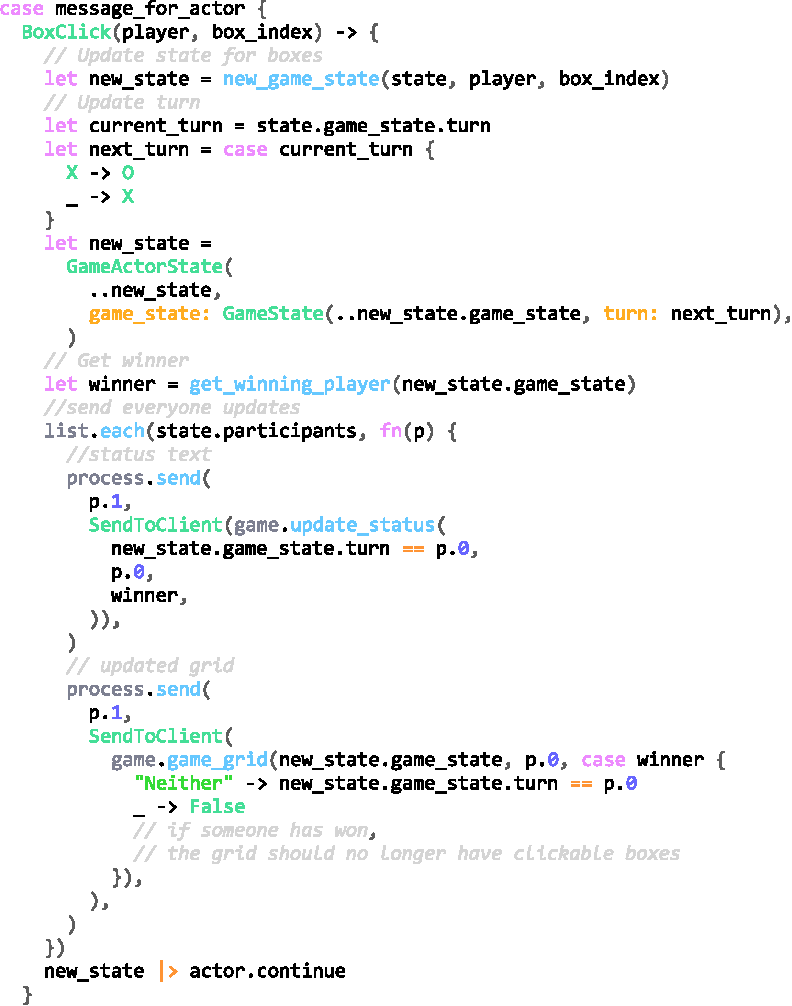
\includegraphics[width=\textwidth]{box_click.pdf}
  \captionof{figure}{The code to handle marking a box on the game board}\label{fig: 9}
\end{minipage}

\newpage

\begin{minipage}[t]{18em}
  In figure \ref{fig: 11}, the \lstinline|get_winning_player| function defines a
  2D list called lines. This list holds lists that contain a possible combination
  of marked boxes that would result in a player winning the game, if they had marked them.
  It checks through all of these combinations using the \lstinline|check_lines| function.
  If a combination has been marked by the same player, the function will return that player,
  to indicate that they have won. Otherwise, it will send \lstinline|Neither| after checking all
  combinations, indicating that either it is a draw or that the game has not ended.
  The \lstinline|get_winning_player| function will check if all boxes have been marked,
  if so the game is a draw, otherwise the game can continue.
\end{minipage}
\hfill
\begin{minipage}[t]{20em}
  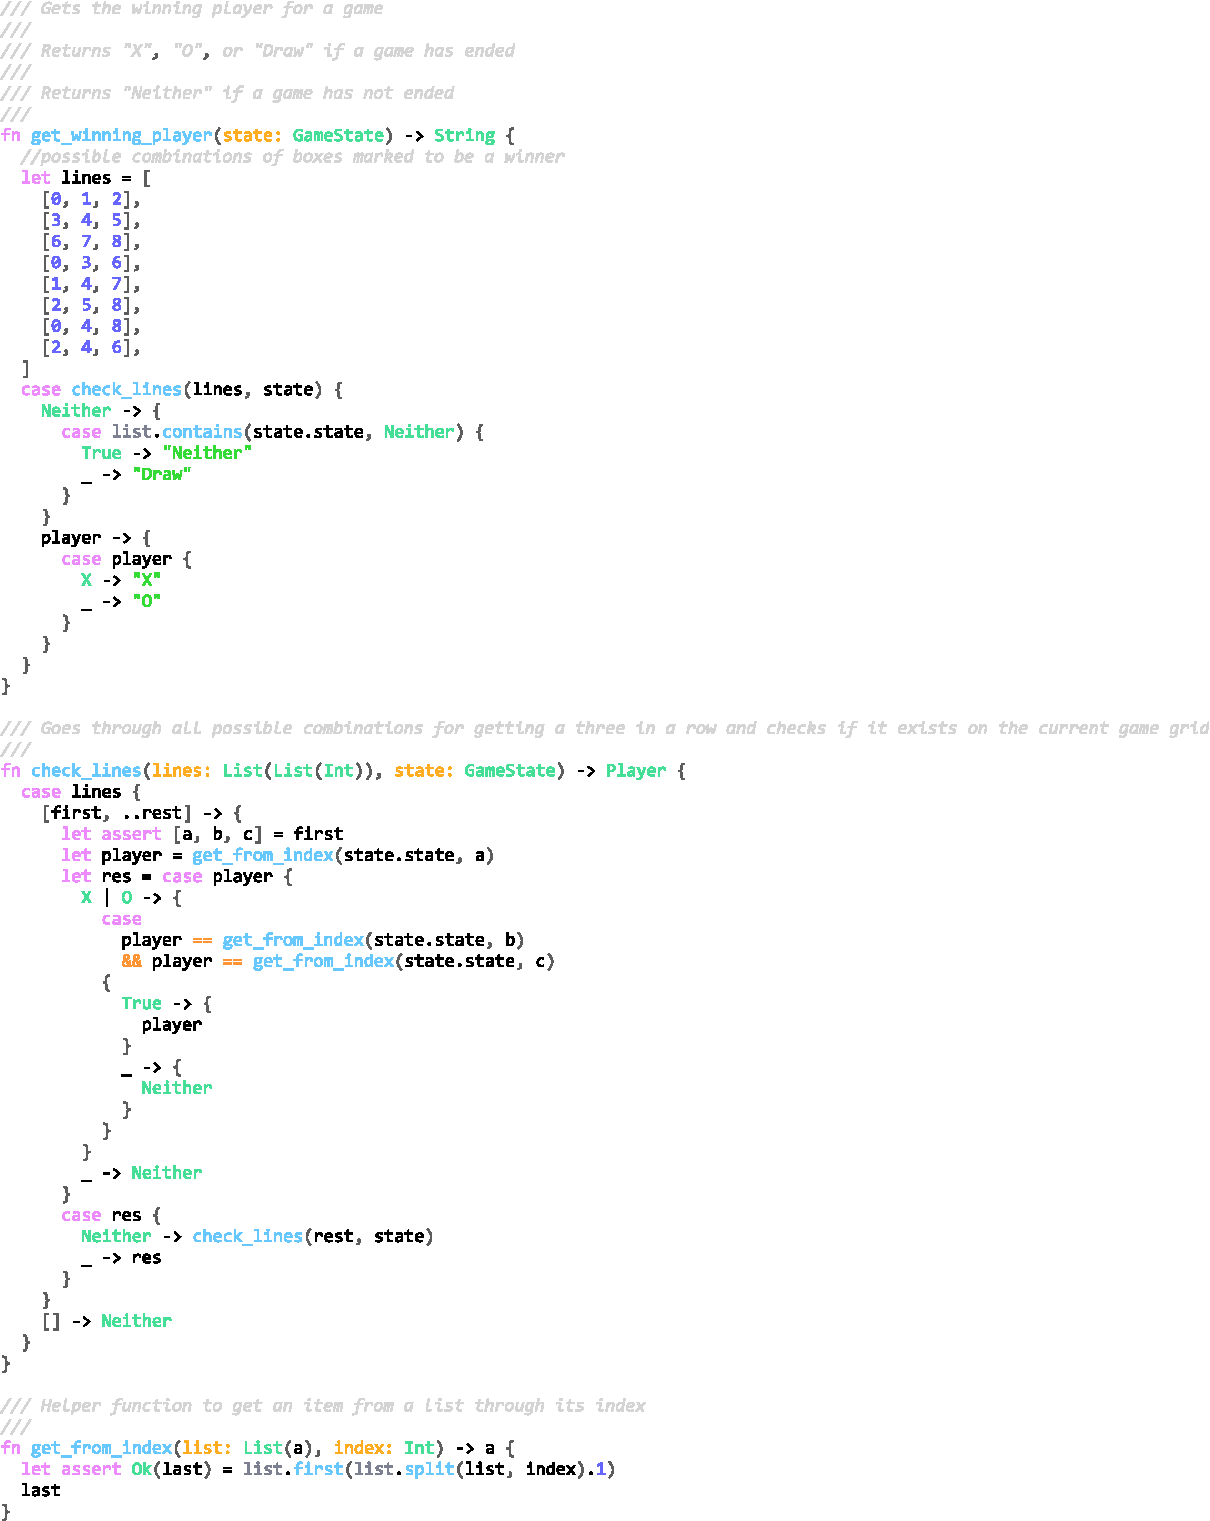
\includegraphics[width=\textwidth]{winning.pdf}
  \captionof{figure}{The functions to check if the game has ended and who won}\label{fig: 11}
\end{minipage}

\section{Challenges faced}

Since every technology in the code stack was new to me, I had to do a lot of learning.
By relying on documentation, and occasionally looking at the source code for
the libraries I was using, I was able to produce proof of concepts that work.
Some libraries, like radish to connect to my Valkey database, did not have
a complete set of capabilities yet, making me have to write extensions to those
libraries within my source code - I contributed the code towards the
library as a result.%https://github.com/massivefermion/radish/pull/7

A major challenge was learning how to implement the actors as I was relying on
the WebSocket actors to communicate with the clients. This was mainly due to the
lack of documentation for this (in otherwise, a fairly well documented library),
within my web framework of choice, mist. \cite{noauthor_example_nodate}.
Thankfully, a user named Connell Reffo figured out how to, within a GitHub issue,
implementing the solution within his Chatter-Reborn project \cite{reffo_connellr023/chatter-reborn_2024}.
This was vital for my progress on creating the prototypes that targeted Erlang and
provided inspiration for how I implemented the actors for my programs. Namely,
using an actor for queues, and then passing the specific scenario, like a chat
room or game, to another actor for the rest of the communications
between users in the scenario.

Another issue was ensuring the correct use of appropriate data structures.
I decided to use an ETS table to manage global state for a server, since the
memory used would sit outside the processes, but within the ERTS, simplifying
the use of the data. I made the table a set, and used a dictionary within the
state for the director actor for the average lookup, insertion and deletion
times of O(1). As well as this, I only used Valkey to store data for the
online chat prototype, as previously mentioned {\hypersetup{linkcolor=teal}(\pageref{valkeyMessageBroker})}, as this meant that I would
only have to rely on it for fast read times, which as previously mentioned {\hypersetup{linkcolor=teal}(\pageref{valkeyRead})},
it delivers.

Other challenges revolved around timing, as would be seen within later sections
of this report. As a result, for my final prototype, the game of Pong, I
modified an implementation of the game from GeeksforGeeks \cite{GeeksforGeeks_pong_2021}, since its sole
purpose was to demonstrate the versatility of the code stack, and as a result
the implementation did not seem too important - as long as it works.

\chapter{A Description of the End Implementation}
Since the prototypes had a modular design that was optimized for the final game,
I reused code from the prototypes, making the final game share a similar,
modular implementation. As a result, I will only focus on the more advanced
aspects of the final game within this section.

\begin{figure*}[ht!]
  \centering
  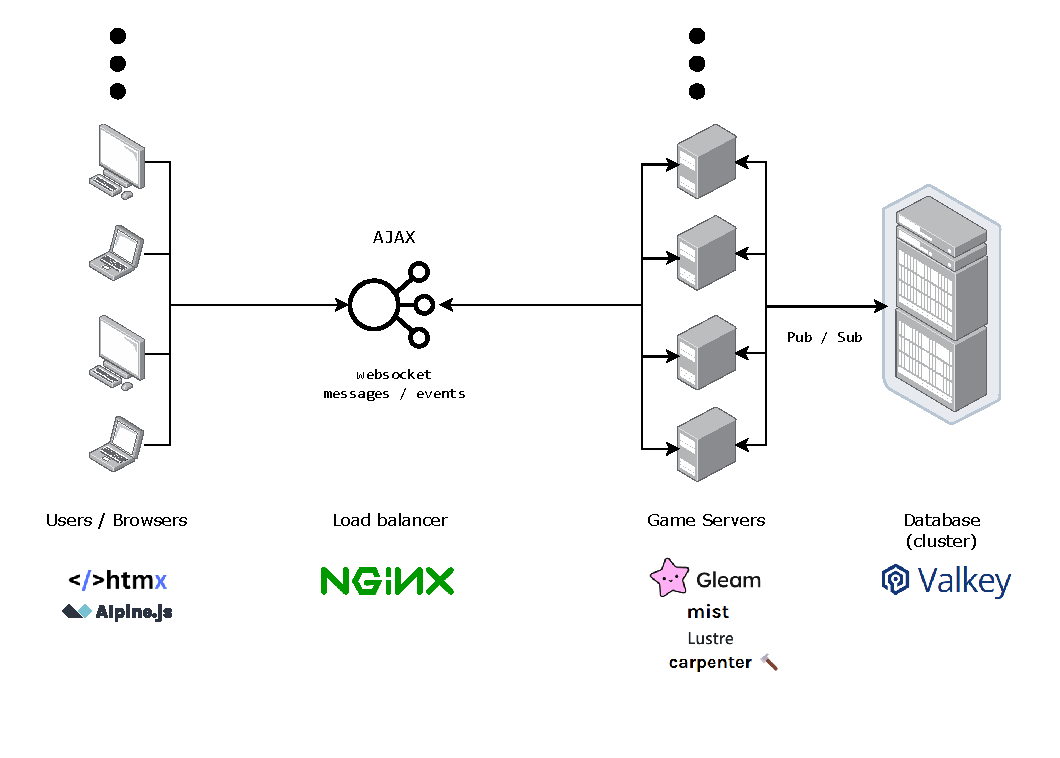
\includegraphics[width=\linewidth]{final_architecture}
  \vspace*{-1.5cm}
  \caption{A diagram representing the game environment architecture I chose to use.}
  \label{fig: 3}
  The use of Alpine.js was explained above {\hypersetup{linkcolor=teal}(\pageref{alpine})}
\end{figure*}

\section{Code implementation}

\addcontentsline{toc}{section}{Overriding actions in progress}
\subsection{Overriding actions in progress}

\addcontentsline{toc}{section}{Racing Actions}
\subsection{Racing actions}
TO ADD

\addcontentsline{toc}{section}{Time-limits for Actions}
\subsection{Time-limits for Actions}
TO ADD

\addcontentsline{toc}{section}{Compound actions}
\subsection{Compound actions}
TO ADD

\addcontentsline{toc}{section}{Realtime dynamic world updates}
\subsection{Realtime dynamic world updates}

\addcontentsline{toc}{section}{Reliability and Error Handling}
\subsection{Reliability and Error Handling}

Aside from using the BEAM for it being a fault-tolerant VM, I implemented some
advanced reliability and error handling features within my code. To start, there
was comprehensive, consistent logging of all data, event, actions, etc. These
logs had comprehensive information and were clear and succinct.

For example, if a UI element did not have use for communicating with the server,
and triggered a message being sent anyway, the following logs would appear on the
server;
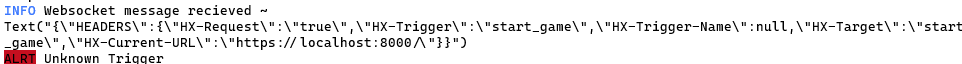
\includegraphics[width=\linewidth]{unknown_trigger_alert.png}

As well as this, I embraced Erlang's 'let it crash' approach to error
handling by letting failing processes crash while supervisors detect and
fix their issues, as previously described {\hypersetup{linkcolor=teal}(\pageref{faultErlang})}.

waiting for join screenshot

\noindent
\begin{minipage}[t]{18em}
  The supervision tree I used for the actors within the final game.
  %\vskip{1em}
  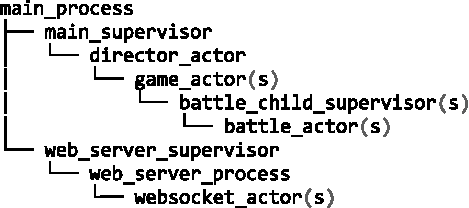
\includegraphics[width=\linewidth]{supervision_tree.pdf}
\end{minipage}
\hfill
\begin{minipage}[t]{20em}
  I.e., the tree could look like the following in deployment (with 2 games being
  played, 5 players in each, and 2 battles occurring in each);
  %\vskip(1em)
  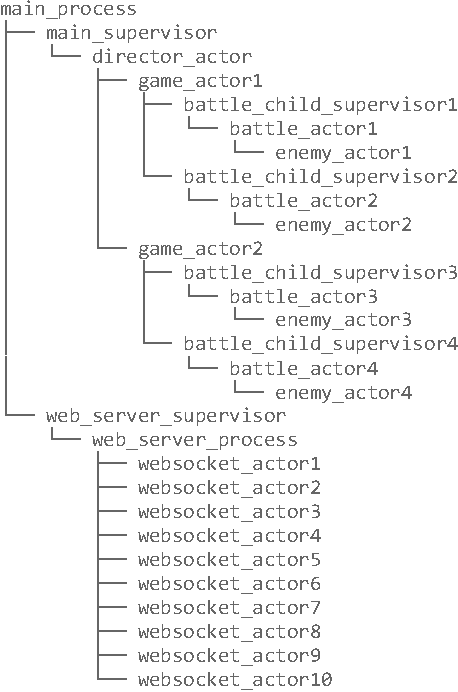
\includegraphics[width=\linewidth]{supervision_tree_deployment_eg.pdf}
\end{minipage}

failed assertion causes panic - image

without a supervisor this would cause the server to stop running completely - image

with supervisors, the director is rescued, and the websocket that triggered
the faulty action can reconnect - add image

Here errors were caused by me purposefuly adding a \lstinline|todo| statement
into a function, causing a \lstinline|panic| and process crash. This was done
for demonstration purposes.

note the large arrays of numbers in the messages will be talked about later in
the report.

error handling, supervisors, tasks, etc.
Split-brain (nodes as cluster, recovery of servers, etc.) - supervisors, let
it fail philosophy

mix concurrency model, barely doing any asny awaiut on js - just client-specific
interactions like oif the user wants to see the leaderboard - game actions all
done on the server

\section{Challenges faced}
hello%TODO
\section{Potential future enhancements}
hi%TODO

ascii encoded messages - 3 screenshots - wisp

\chapter{Planning and Time-scale}

The following is what was planned for the project;

Term 1:\\\\
\scalebox{1}{
  \begin{tabular}{r |@{\bulletPoint} l}
    Week 1 - 2   & Produce the project plan \& research on viable technologies for use              \\
    Week 3       & Plan final game screens, structure, features, etc.                               \\
    Week 4       & Decide on the technologies to use and build the fundamental architecture         \\
    Week 5       & Online chat                                                                      \\
                 & Build a proof of concept that exhibits the behaviour of concurrent execution     \\
    Week 6       & Tic-Tac-Toe                                                                      \\
                 & Build a proof of concept board game that can have multiple games played at once  \\
    Week 7       & Pong                                                                             \\
                 & Build another proof of concept game to test the modularity of my technologies    \\
    Week 8       & Evaluate the proof of concepts \& build the basis of the final game              \\
    Week 9       & Produce a survey report on game environments                                     \\
                 & Produce a report describing the implementations of the proof of concepts         \\
    Week 10 - 11 & Implement the foundational concurrent features for the final game;               \\
                 & Ensure multiple games can be played at the same time                             \\
                 & Ensure multiple players can play a game together                                 \\
                 & Ensure the players, within a game, can trigger multiple actions at the same time \\
                 & Ensure error reporting procedures are provided                                   \\
  \end{tabular}
}

Term 2:\\\\
\scalebox{1}{
  \begin{tabular}{r |@{\bulletPoint} l}
    Week 1 - 2   & Refine and optimize the features implemented at the end of the first term   \\
                 & Week 1 - Client-side improvements                                           \\
                 & Week 2 - Server-side improvements                                           \\
    Week 3 - 4   & Implement additional game features (niceties) and polish the user interface \\
                 & Implement the chat room (real-time communication)                           \\
                 & Implement the map (real-time dynamic world updates)                         \\
                 & Implement an information section in the game (real-time updates)            \\
                 & (Content set individually, for each player, based on alliances, etc.)       \\
    Week 5 - 6   & Conduct thorough performance testing and optimize for scalability           \\
    Week 7       & Implement improvements to reliability and error handling                    \\
    Week 8       & User testing and gathering feedback                                         \\
    Week 9       & Address feedback and make final adjustments                                 \\
    Week 10 - 11 & Prepare the final documentation, presentation and project report            \\
  \end{tabular}
}

As can be seen from my diary below, I occasionally deviated from the plan due
to timing issues, but I still managed to deliver everything.

\newpage

\chapter{Professional considerations for the project}

During the development of the project, I had to carefully consider many
professional issues that could have potential long-term implications.
This was especially due to the fact that I decided to learn completely
new technologies for my entire tech stack, which meant that I relied
on modern technologies that were unfamiliar to me at the conception of what
the project would entail. This decision, while making the project challenging,
allowed me to expand my skill set and adapt to industry trends,
aligning with the BCS Code of Conduct, particularly the section on
Professional competence and integrity, which emphasizes the need to
"develop your professional knowledge, skills and competence on a continuing
basis, maintaining awareness of technological developments, procedures,
and standards that are relevant to your field".

%TODO cite https://www.bcs.org/membership-and-registrations/become-a-member/bcs-code-of-conduct/

One of my concerns was the licensing of the different products I was using.
While all of it was open source, they, for e.g., Gleam, NGINX, and Valkey,
each have their own licenses.
While they all generally permit free use, modification, and distribution,
some had extra requirements that were important to meet,
such as proper attribution and the inclusion of license notices in
the project, which was especially the case for more creative works used
like the icons and fonts for my game UIs.

Not meeting these requirements
could lead to the inability to commercialize the project
in the future, and legal disputes, especially since some of my prototypes are
already being hosted. To meet them, I, for e.g., decided to add 'information' sections on
the games which provide the proper attribution of any product I used. I
also added comments in my code, wherever I took inspiration from, or directly
used something I found online, in an attempt to avoid unintentional plagiarism.

%TODO link?
%TODO information modal image

The issue of licensing is a broad one, with many issues that may arise.
For example, Redis Labs infamously faced backlash when it applied
the Commons Clause to a set of modules, and extensions to the core Redis database.
This overrode the existing open source license "to render the
software effectively proprietary and source available while still leveraging
the brand of the original open source license"

%TODO cite https://redmonk.com/sogrady/2024/07/16/post-valkey-world/

This decision raised questions about the sustainability of open-source projects
and the balance between community contributions and commercial interests.
This example highlighted the importance of understanding
and respecting licensing terms, as well as considering the long-term
implications of relying on open-source technologies. Thankfully, in the example's
case, Valkey, the database I chose for this project, had a meaningful role.
The Valkey project came together unusually quickly, recieving a suprising amount
of attention, ending up as the leading alternative to Redis. Since it is a fork
of Redis OSS, developers could use the same drivers as those with Redis, meaning
that no changes to apps were required to switch to Valkey.

%TODO cite https://redmonk.com/sogrady/2024/07/16/post-valkey-world/

Another quick note to make is that, while I was using Gleam, which is open source,
if I was using proprietary, new technologies, this project would have been a lot
more difficult as I sometimes had to look at the source code of the libraries I was using
due to immature and sometimes completely absent documentation. Understanding how
to use a product by looking at it's internals like this, may count towards
reverse engineering, which may be against the licence used for a proprietary
product.

Another issue was usability and accessibility.
Ensuring that the games are accessible to a diverse
audience, including those with disabilities, is not only a professional
responsibility but also a moral one. For example, incorporating features like
keyboard navigation, screen reader compatibility, and colorblind-friendly
design would make the game more inclusive.

Ignoring these aspects could
alienate potential players and lead to criticism or worse, health effects, as
seen in the backlash against games like Cyberpunk 2077, which not only lacked
sufficient accessibility options but also lacked warnings that the game
may cause seizures. The developers had to roll out updates which later added
these warnings.%TODO cite https://www.polygon.com/2020/12/8/22163153/cyberpunk-2077-accessibility-epilepsy-seizure-warning
The game was also criticized for being poorly optimized,
resulting in a subpar experience for many players.
%https://steamcommunity.com/app/1091500/discussions/7/4428814589383884489/
%https://expertbeacon.com/why-does-my-cyberpunk-run-so-bad/

In my project, I focused primarily on server architecture and concurrency,
which meant that optimization for client-side performance was not a
priority. As a result, I used libraries like TailwindCSS directly from
their CDN, which gives me a warning in my console.%TODO image
However, this decision could have practical implications,
as poorly optimized games can lead to negative user experiences and
damage the reputation of the developers. This serves as a reminder
of the importance of balancing backend and frontend development to
deliver a polished and accessible product. To make the game ready for
deployment, I would need to account for this accessibility issue and optimize for production
by, in this example, utilizing the Tailwind CLI, which would scan my source files for
classes and build only the CSS I would need, reducing the size of
the download.

Browsers are inherently designed with accessibility in mind, as they serve
as a universal platform for users across a wide range of devices and
abilities, which is why I chose to make the games browser-based rather than
developing desktop or mobile apps. This decision not only ensures broader
accessibility but also leverages the built-in tools and standards that
browsers provide, such as screen reader compatibility and keyboard navigation,
making it easier to address accessibility concerns and deliver a more
inclusive experience.

Addressing these professional issues has been a valuable learning experience.
It has taught me the importance of considering the broader societal and
ethical implications of software development, beyond just technical
functionality. By proactively addressing issues, that are not limited to
licensing and accessibility concerns, I have not only ensured the integrity of my
project but also developed a deeper understanding of the responsibilities
that come with being a software engineer. These lessons will
undoubtedly inform my approach to future projects and my professional
practice as a whole.

\chapter{Reflection / self-evaluation}

As previously mentioned {\hypersetup{linkcolor=teal}(\pageref{valkeyMessageBroker})}, and as can be seen within my project diary below,
I have completed all of my goals for the project.
The project was highly successful; I implementing a concurrent game environment
using OTP and Gleam, developed functional prototypes (online chat, Tic-Tac-Toe,
Pong), and creating a final game with advanced concurrency features.
Despite challenges, like learning new technologies and managing time
constraints, the produced architecture and software design ensured
scalability and fault tolerance.
There were many key aspects that went right; choosing Erlang’s actor model
and Gleam’s tooling streamlined development,
the pool architecture with Pub/Sub ensured scalability without Kubernetes’
complexity and thorough documentation and testing enhanced reliability.

However, the project (and its plan) did have it's issues.
I had underestimated how much time it would
take to carry out extensive research and learn all of the new technologies. This
coupled with my many other commitments mentioned within the risks in my project plan,
meant that I could not use the time I had initially planned on allocating towards
creating my games and their environments. I had also experienced some hardware
issues and unexpected challenges when moving between frameworks / the compilation
targets, which should have been identified and planned for. I had also not planned to
produce an interim report, which has taken a significant amount of time.
The result of all of this can be seen within the
code for the project, specifically the game of pong, and tests. While I tried to make tests comprehensive,
and ensured that all code is working through play-testing, the tests leave out
some edge cases, leaving possible bugs in the codebase.
To add, planning the final game screens, its structure, and features, etc., before
deciding on the technologies to use and producing the prototypes was not helpful and
did not make sense to do, since some of my expectations and plans had to change as I
made decisions and produced code.

Future work could expand the game’s features (e.g., cross-region replication) or
explore Kubernetes integration for large-scale deployment.
Projects rarely go exactly to plan, and through this one I have learnt a lot.
To start, future projects need buffer time for experimentation and debugging new
technologies. As well as this, focusing on core functionality like the game
server’s concurrency model before polishing niceties, like the GUI, ensured the
architecture was solid. Building modular, reusable components streamlined
prototyping and simplified scaling later, saving me time.
Documenting code and my decisions was also crucial, preventing moments
where I cannot recall the purpose of a module or function after a significant
break from a feature.

\newpage
\addcontentsline{toc}{chapter}{Bibliography}
\bibliography{refs}

\chapter{Appendix}
\section{Diary}
%TODO add new stuff
Taken from the git repository and modified to be suitable for pdf format.

TO ADD
% add here (maybe convert md to pdf and includegraphics - easier & can remove toc limit)

\section{Video Demo}
TO ADD

%cite properly
The demo video can be found at the following link; \href{}{VIDEO}

This video used a text-to-speech engine by elevenlabs \cite{noauthor_ai_nodate}.

\section{Screenshots}
Images for all prototypes \& the final game
\addcontentsline{toc}{section}{Prototype 1 - Online chat}
\subsection{Prototype 1 - Online chat}
This was produced to target JavaScript and Erlang%TODO

TO ADD
\addcontentsline{toc}{section}{Prototype 2 - Tic-Tac-Toe}
\subsection{Prototype 2 - Tic-Tac-Toe}
This was produced to target JavaScript and Erlang%TODO

TO ADD
\addcontentsline{toc}{section}{Prototype 3 - Pong}
\subsection{Prototype 3 - Pong}
This was produced to target Erlang%TODO

TO ADD
\addcontentsline{toc}{section}{Final game - Zarlasht}
\subsection{Final game - Zarlasht}
This was produced to target Erlang%TODO

TO ADD
\chapter{Acronyms \& Glossary}
%TODO add new stuff
Threads

A sequential flow of control within a process. A process can contain one or more threads.
Threads have their own program counter and register values, but they share the memory space
and other resources of the process

Parallelism

Truly simultaneous execution or evaluation of things

Concurrency

The coordination and management of independent lines of execution. These executions
can be truly parallel or simply be managed by interleaving. They can communicate
via shared memory or message passing. (Rob Pike's definition: “the composition of
dependently executing computations”)

Deadlock

Two threads are blocked, waiting for each other to release a resource that they need. So neither can proceed

Starvation

A thread is waiting for a resource that is always given to other threads

Livelock

Two threads are waiting for each other to release a resource. They keep trying to resolve their impasse, but never succeed

Race Condition

Two threads are trying to access a shared resource at the same time. The result is dependent on the order of execution

BEAM

Bogdan's Erlang Abstract Machine / Björn's Erlang Abstract Machine - a virtual machine, built into the OTP
distribution, that executes user code in the ERTS

OTP

Open Telecom Platform - a framework that provides an abstraction of common uses of / interactions with
certain types of processes. It provides modules and behaviours that represent standard implementations of
common practices like process supervision, message passing, spawning tasks, etc.

ERTS

Erlang Run Time System - the system that contains functionality necessary to run the Erlang system

OS

Operating System - system software that manages computer hardware and software resources, and
provides common services for computer programs

WebSockets

A computer communications protocol, providing a simultaneous two-way communication channel
over a single TCP connection

TCP

Transmission Control Protocol - one of the main protocols of the Internet protocol suite. TCP provides
reliable, ordered, and error-checked delivery of a stream of bytes between applications over a IP network

HTTP

HyperText Transfer Protocol - an application layer protocol in the Internet protocol suite.
It is used for transferring data between clients and servers

DoS

Denial of Service - An attack where the perpetrator seeks to make a machine or network resource unavailable
to its intended users

DDoS

Distributed Denial of Service attack - a DOS with traffic from multiple sources

GUI

Graphical User Interface that allows users to interact with systems through mechanisms like buttons, windows, etc.

OSS

Open-Source Software that is freely available and can be modified and redistributed by anyone

API

Application Programming Interface - defines how different software components should interact

DRM

Digital Rights Management - technology that controls access and usage of digital content

CAP

Consistency, Availability, Partition Tolerance theorem, describing trade-offs in distributed system design

I/O

Input / Output process for communication between a computer system and the outside world

XML

Extensible Markup Language - used to structure data

AJAX

Asynchronous JavaScript and XML - used for creating fast and dynamic web pages

XMLHttpRequest

A web API for transferring data between a web browser and web server

UML

Unified Modeling Language - a standard that includes many types of diagrams that help visualizing software and system design

TDD

Test-Driven Development - a methodology of writing tests before actual code implementation

HTML

Hypertext Markup Language - used to define the structure of web pages

IP

Internet Protocol - for routing data packets across networks

CSS

Cascading Style Sheets - used for styling web pages

FFI

Foreign Function Interface - used for calling functions written in other programming languages

URL

Uniform Resource Locator - used for specifying the address of resources on the internet

JSON

JavaScript Object Notation - often used for lightweight data interchange and storage

PoC

Proof of Concept - a demonstration of a concept

\end{document}
\end{article}